% Numbers: ../notes/replication-results.md; raw data: ../results/*.jsonl; figures made by
% ../code/scripts/article_figures.py and make_figures.py.

\section*{Introduction}

Bou Diab, Chammas and Daou\supercite{BouDiab2025} proposed a conductance-based network model of
the songbird premotor nucleus HVC. It combines HVC\textsubscript{RA} and HVC\textsubscript{X}
projection neurons with interneurons (HVC\textsubscript{INT}). The single-cell models come from
Daou et al.\supercite{Daou2013}, and the synapses are kinetic AMPA and GABA\textsubscript{A}
synapses\supercite{Destexhe1994}. A feed-forward chain of 20 microcircuits with structured
inhibition reproduces the ultra-sparse HVC\textsubscript{RA} bursts seen in
vivo\supercite{Hahnloser2002}, the 1--4 rebound bursts of HVC\textsubscript{X}
neurons\supercite{Kozhevnikov2007} and dense interneuron firing. Single-neuron changes in $I_A$,
$I_{SK}$, $I_{CaT}$ or $I_H$ break the sequence.

We reimplemented the model independently in Python from the article text, and report which
results can be reproduced.

\section*{Methods}

\subsection*{Independence protocol}
We worked in two phases, each closed by a git tag before the next began:
\begin{enumerate}
\item \textbf{Text only.} The article (text, Appendix~1, figures) and the papers it cites for the
  single-cell models: Daou et al.\supercite{Daou2013} and that paper's published code. The
  authors' supplementary code was downloaded but left unopened, with its SHA-256 checksums
  recorded (tag \texttt{phase1-complete}).
\item \textbf{Comparison with the supplementary code} (tag \texttt{phase2-complete}).
\end{enumerate}
The replication therefore tests what can be reproduced from the published description: the
article, its supplement and the work it cites. We did not use unpublished information from the
original authors. We also searched ModelDB, GitHub, Zenodo, Figshare, OSF and the authors' lab
website for the network code, which the article says will be deposited on ModelDB, and did not
find it.
Every parameter is tagged in the code with its source: the article, Daou 2013 text, Daou 2013
code, or our choice.

\subsection*{Model and corrections}
The equations follow Appendix~1 of the original, with the corrections in
Table~\ref{tab:issues}. These come from the Daou et al.\ paper and code, or are required for
physically meaningful behaviour. The most consequential is the potassium activation time
constant. With the printed constant $\tau_n = 10$\,ms, every action potential is
$\sim$10\,ms wide and HVC\textsubscript{RA} cannot burst. The voltage-dependent form of Daou et
al.\ restores normal spikes.

\subsection*{Implementation}
The network is one vectorised ODE system of 2487 variables. It is integrated with SciPy's
Dormand--Prince RK45\supercite{Dormand1980,Virtanen2020}, the method behind MATLAB
\texttt{ode45}, at rtol $10^{-6}$ and atol $10^{-9}$. These tolerances are tighter than
MATLAB's defaults; see Robustness. Fixed-step RK4 is used for comparison and for noise. The
network is built by the article's rules. Open choices are listed in Table~\ref{tab:issues}:
\begin{itemize}
\item per-microcircuit counts are sampled to sum to 120/50/50;
\item interneuron inputs are drawn from the whole HVC\textsubscript{RA} pool;
\item the sequence starts with a 500\,pA, 10\,ms pulse into the first HVC\textsubscript{RA}.
\end{itemize}
Code, configurations, raw results and the full issues log are at
\url{https://github.com/sheetal-jadhav/rescience-zeina-boudiab-2025-hvc}. All tests (\texttt{pytest}) and
figures can be regenerated with the scripts in \texttt{code/scripts} (order in the README).

\subsection*{Second implementation in Brian2}
To check our implementation, we wrote the model a second time in Brian2\supercite{Stimberg2019}
(\texttt{code/hvcnet\_brian2}). The equations are rewritten in Brian2's equation syntax, with
units, from the same specification. Only the parameter values and the network wiring are
shared, so both codes simulate identical networks. Brian2 integrates with fixed-step RK4
(0.01\,ms) and updates synapses and neurons in separate sub-steps. The folder has its own
README, requirements and a single script that runs the test, the cross-check and the comparison
with the original article.

\subsection*{Parameters not given in the article}
The article gives the variable conductances only as allowed ranges (Fig.~13). We sampled 200
configurations uniformly inside those ranges and kept the one maximising
\[
N_{RA,\text{ok}} - 20\,|\bar{n}_\text{spk} - 4.76| - 10\,|\bar{d}_\text{burst} - 8.12\,\text{ms}|,
\]
where $N_{RA,\text{ok}}$ counts HVC\textsubscript{RA} that fire one burst of 3--6 spikes lasting
at most 10\,ms (the article's criterion). The objective uses HVC\textsubscript{RA} only, because
no sampled configuration met the HVC\textsubscript{X} criterion.

\section*{Results}

Figures~\ref{fig:2}--\ref{fig:13} are laid out like the original Figures~2 and 4--13. Neuron
indices refer to our network instance.

\subsection*{Fig.~2 matches only with the Mooney \& Prather procedure and fitted pair synapses}
We simulated the stimulated cell of each Fig.~2 panel on its own, with two protocols
(Fig.~\ref{fig:2}). With the stimulus stated for the model (0.5\,nA, 10\,ms pulses; a 0.5\,nA,
500\,ms step in D), HVC\textsubscript{RA} fired 3 spikes per pulse and interneurons 2, against one
each in the original, and the interneuron in D fired at 178\,Hz, against $\sim$60\,Hz (50 spikes
over the $\sim$820\,ms step drawn in the original; the text says 500\,ms). This is not specific to
our implementation. A Python port of the authors' own Fig.~2 cell code gives the same 176\,Hz
interneuron, and its HVC\textsubscript{RA} cell does not fire at all to the stated pulse. Removing
$I_{KNa}$ and $I_{NaP}$, which that code contains and the article excludes, changes neither result.
For HVC\textsubscript{RA} the A-type conductance decides the spike count: one spike needs
$g_A\approx 80$--90\,nS, outside the published range of 1--14\,nS.

Mooney and Prather adjusted the current or the resting potential of the stimulated cell
``to elicit only a single action potential per pulse''\supercite{MooneyPrather2005}. A holding
current cannot do this for our HVC\textsubscript{RA} (3 spikes from $-74$ to $-98$\,mV), so we
adjusted the amplitude, taking the middle of each cell's one-spike range: 150\,pA for
HVC\textsubscript{RA}, 250\,pA for interneurons, and 500\,pA for HVC\textsubscript{X}, which needs
no change. For D we used 145\,pA for 820\,ms. With this procedure every stimulated cell fires one
spike per pulse, HVC\textsubscript{RA} with the small after-depolarisation seen in the original,
and the interneuron in D fires 49 spikes at 60\,Hz. These amplitudes are below the 0.5--1\,nA used
in slices, which we attribute to the higher input resistance of the model cells.

The pair conductances of Fig.~2 were calibrated by eye and are not reported. We fitted them to
the original model traces, measured with their scale bars: INT$\to$X 10\,nS (IPSP 4.1\,mV, target
4.0), X$\to$INT 11\,nS (one interneuron spike per HVC\textsubscript{X} spike), and RA$\to$INT
25\,nS in A (one interneuron spike per HVC\textsubscript{RA} spike) but 7.4\,nS in B (a
subthreshold 6.6\,mV EPSP, target 6.5). A and B need different RA$\to$INT strengths, as in Mooney
and Prather's own sub- and suprathreshold pairs. The network uses 21--27\,nS for the same
connections. Two traces were not fitted and serve as tests: the disynaptic IPSP in A is
3.7--4.2\,mV (target $\sim$4.7) and the HVC\textsubscript{X} hyperpolarisation in D is 5.2\,mV
(target 4.7--5), with the same ripple at each interneuron spike (Fig.~\ref{fig:2}, right). Three
features are not reproduced: the interneuron spike on the second pulse in B (identical pulses on a
settled cell give identical EPSPs), the absence of an HVC\textsubscript{X} rebound spike after the
step in D (ours fires one, 66\,ms after the step), and a small depolarisation after each
interneuron spike in C. With the stated 0.5\,nA and the same synapses, the extra presynaptic spikes
roughly double the postsynaptic responses (Fig.~\ref{fig:2}, left).

\subsection*{Sequence propagation is reproduced (Fig.~4)}
In 50 of 50 random network instances, activity propagated through all 120
HVC\textsubscript{RA} in chain order (Fig.~\ref{fig:4}). Bursts had $3.93\pm0.12$ spikes and
lasted $8.61\pm0.35$\,ms, against $4.76\pm0.48$ and $8.12\pm0.89$\,ms in the original. On
average 115 of 120 HVC\textsubscript{RA} met the article's burst criterion. Successive neurons
fired 1.96\,ms apart.

The burst statistics do not match both original values at once. In our model, burst size and
duration move together: across 200 configurations inside the published ranges they correlate at
0.99, and configurations with the original's $\sim$4.8 spikes last $\sim$11.5\,ms
(Fig.~\ref{fig:4tradeoff}A). Our spikes are $\sim$2.9\,ms apart within a burst, against
$\sim$2.2\,ms in the original. Neither the start pulse nor the wiring explains this. Once the first
neuron bursts, the chain settles at $\sim$4 spikes per burst within two or three links for any
start pulse from 250 to 800\,pA (with 150\,pA, the Fig.~2 amplitude, single spikes propagate
instead). The Fig.~2 pair conductances and the stated wiring rules change burst size by less than
0.1 spike. The wiring does not enforce the stated rule that no inhibition reaches an
HVC\textsubscript{RA} neuron during its burst: interneurons receive input from any microcircuit,
and in one network 31\% of interneuron$\to$RA synapses deliver inhibition during the target's
burst. Of the spike-shaping parameters we tested, only the HVC\textsubscript{RA} capacitance,
which the original does not report, shortens the interval within bursts. With 16\,pF instead of
the 20\,pF of Daou et al.\supercite{Daou2013}, and $g_{SK}$ and $g_A$ at the top of their published
ranges, bursts had $4.34\pm0.21$ spikes and lasted $9.01\pm0.66$\,ms (10 networks), both within
one standard deviation of the original, and successive neurons fired 1.64\,ms apart. The cost is
that only 78 of 120 HVC\textsubscript{RA} met the burst criterion (Fig.~\ref{fig:4tradeoff}B).
We therefore keep 20\,pF for all figures and report this as a sensitivity result.

\subsection*{Inter-burst delay is reproduced in direction only (Fig.~5)}
Raising $g_{AMPA}$ from 10 to 12\,nS shortened the delay from 5.6 to 4.6\,ms and added a spike,
as the original text states. The original Fig.~5A legend shows the opposite. Raising $g_A$ from
10 to 13\,nS lengthened the delay by only 0.2\,ms, against $\sim$3.6\,ms in the original, and the
postsynaptic burst had 1--2 spikes rather than $\sim$6 (Fig.~\ref{fig:5}).

\subsection*{HVC\textsubscript{X} and interneuron firing are not reproduced from the published description (Figs.~7, 8, 10)}
Across 200 calibration runs inside the published ranges, every equation variant found in the
supplementary code, and capacitance variations, HVC\textsubscript{X} never fired multi-spike
rebound bursts. They fired single rebound spikes, and 27 of 50 were silent
(Figs.~\ref{fig:7}, \ref{fig:10}). Interneurons fired sparsely (median 8 spikes per 400\,ms)
rather than in the dense bursts of the original Figs.~7A and 8 (Fig.~\ref{fig:8}).

In isolation, our HVC\textsubscript{X} model cannot fire faster than $\sim$160\,Hz, whereas the
original Fig.~10 shows rebound bursts at $\sim$500\,Hz. An exploratory test of single changes,
far outside the published values, also produced no bursts: faster $I_{CaT}$ de-inactivation, a
hyperpolarising bias current, 3$\times$ stronger interneuron drive, and 6$\times$ stronger or
8$\times$ longer inhibition.

The supplementary single-cell file contains two currents that the article says were removed
($I_{NaP}$, $I_{KNa}$), so we also tested the complete HVC\textsubscript{X} model of Daou et
al.\supercite{Daou2013}, read directly from its published XPP files. It fired at most
$\sim$100\,Hz (37\,Hz for the published 150\,pA step) and 60--86\,Hz after release from a long
hyperpolarisation. It gave no rebound at all after a 50\,ms hyperpolarising pulse, which mimics
an inhibitory volley (\texttt{code/scripts/daou13\_xcell.py}). Neither the published reduced
cell nor the full 2013 cell produces the original's HVC\textsubscript{X} phenotype. The
HVC\textsubscript{X} parameters used in the original network therefore appear to differ from all
published ones. One possible source is the fits of Daou \& Margoliash\supercite{DaouMargoliash2020},
which the article cites to justify identical HVC\textsubscript{X} properties, but those
parameters are not reported.

\subsection*{The sequence is far more robust to single-neuron changes than reported (Figs.~6, 9, 11, 12)}
\begin{itemize}
\item \textbf{HVC\textsubscript{RA} (Fig.~6).} Raising $g_A$ up to 3$\times$, or $g_{SK}$
  15$\times$ (the original's factor), never broke the chain (0/16). With inhibition at the top of
  its range (5\,nS), $g_A$ $\times$20 or $g_{SK}$ $\times$60 silenced the perturbed neuron and
  broke the chain there, 8/8. At that inhibition, $g_{SK}$ $\times$15 broke the chain in 1 of 8
  trials, four neurons downstream of the perturbed one (Fig.~\ref{fig:6}).
\item \textbf{Interneurons (Fig.~9) and HVC\textsubscript{X} (Fig.~11).} The perturbed cells
  fired more, but the chain never broke (0/24 for each figure; Figs.~\ref{fig:9},
  \ref{fig:11}).
\item \textbf{HVC\textsubscript{X} variation (Fig.~12).} Drawing HVC\textsubscript{X}
  conductances per neuron broke the chain in 0 of 100 runs, against 59/100 disrupted in the
  original (Fig.~\ref{fig:12}).
\end{itemize}
In the original, these breaks run through dense interneuron firing, which we do not reproduce.

\subsection*{The narrow HVC\textsubscript{RA}$\to$HVC\textsubscript{RA} window is reproduced (Fig.~13)}
Varying one conductance at a time (Fig.~\ref{fig:13}):
\begin{itemize}
\item HVC\textsubscript{RA}$\to$HVC\textsubscript{RA} worked only between 28.0 and 30.5\,nS,
  matching the original's narrow 29--31\,nS. Weaker synapses broke the chain; stronger ones gave
  over-long bursts.
\item HVC\textsubscript{RA} also required $g_{SK}\geq{\sim}11.6$\,nS and $g_A\geq{\sim}5.6$\,nS. These
  are only the upper parts of the published ranges, so drawing conductances per neuron across the
  full ranges left just 7/120 HVC\textsubscript{RA} meeting the criterion.
\item All HVC\textsubscript{X} and interneuron conductances, and the remaining synapses, were
  tolerated across and beyond their ranges, consistent with the chain's insensitivity to those
  cells.
\end{itemize}

\subsection*{Robustness}
\begin{itemize}
\item \textbf{Solver tolerance} (Fig.~\ref{fig:num}). At MATLAB's default tolerances, spike times
  drifted by up to $\sim$8\,ms along the chain, bursts lengthened from 8.6 to 10.9\,ms, and the
  burst criterion dropped from 115 to 44 of 120. RK4 at 0.025 and 0.01\,ms agreed with tight
  RK45 to within 0.4 and 0.03\,ms.
\item \textbf{Noise.} Additive white-noise current had no effect up to
  $\sigma=10$\,pA\,ms$^{1/2}$. It degraded bursts progressively above that and broke the chain
  at $\sigma=160$.
\item \textbf{Removing HVC\textsubscript{X}} entirely, a question raised in review of the
  original, left propagation intact (16/16; 115/120 meeting the criterion).
\end{itemize}

\subsection*{The Brian2 implementation reaches the same verdict (Table~\ref{tab:brian2})}
Isolated HVC\textsubscript{X} and interneurons agree between the two codes to within 0.03\,ms
over 1.5\,s. On a small test network, every neuron has the same spike count in both codes, and
the remaining timing difference halves when Brian2's step is halved. Across networks, the two
codes give the same statistics for every measure we compare with the original
(Table~\ref{tab:brian2}). The cross-check also exposed an error of ours: the pre-stimulus
settling had run at SciPy's default tolerance, which shifted the spontaneous
HVC\textsubscript{X} and interneuron activity. All results reported here were rerun after the
fix.

\begin{table}[h]\small
\caption{Original article vs our two implementations. Mean $\pm$ SD across networks: 50 wiring
seeds (rows 1--7), 16 without HVC\textsubscript{X}, 100 runs for Fig.~12.}
\label{tab:brian2}
\begin{tabular}{p{0.42\linewidth}p{0.16\linewidth}p{0.16\linewidth}p{0.16\linewidth}}
\hline
Measure & Original & SciPy & Brian2 \\ \hline
Chain completes, in order (Fig.~4) & yes & 50/50 & 50/50 \\
HVC\textsubscript{RA} spikes per burst & $4.76\pm0.48$ & $3.93\pm0.12$ & $3.93\pm0.15$ \\
HVC\textsubscript{RA} burst duration (ms) & $8.12\pm0.89$ & $8.61\pm0.35$ & $8.57\pm0.44$ \\
HVC\textsubscript{RA} meeting the burst criterion (of 120) & 120 & $114.9\pm1.9$ & $114.9\pm2.1$ \\
HVC\textsubscript{X} meeting the burst criterion (Figs.~7B, 10) & all & 0/2500 & 0/2500 \\
HVC\textsubscript{X} spikes per burst (median) & 4--9 & 1 & 1 \\
Interneuron spikes per 400\,ms (median; Figs.~7A, 8) & dense & 8 & 8 \\
HVC\textsubscript{X} removed: chain completes & not tested & 16/16 & 16/16 \\
Per-neuron HVC\textsubscript{X} variation: chain broken (Fig.~12) & 59/100 disrupted & 0/100 & 0/100 \\ \hline
\end{tabular}
\end{table}

\section*{Discussion}

\paragraph{What reproduces.} The core mechanism reproduces from the text plus Daou et
al.\supercite{Daou2013}: a chain of single-compartment HVC\textsubscript{RA} neurons coupled by
AMPA synapses propagates sparse, stereotyped bursts. This holds in every random network instance
we built, for every equation variant we tried, and with HVC\textsubscript{X} removed. The narrow
working window for HVC\textsubscript{RA}$\to$HVC\textsubscript{RA} conductance also reproduces,
within 1\,nS.

\paragraph{What does not.} The parts of the original that involve HVC\textsubscript{X} and
interneurons do not reproduce from the published description:
\begin{itemize}
\item HVC\textsubscript{X} rebound bursts (Figs.~7B, 10);
\item dense interneuron bursting (Figs.~7A, 8);
\item Fig.~2 at the stated 0.5\,nA (it matches, apart from three details, only when the current is
  adjusted as in Mooney \& Prather and the unreported pair conductances are fitted);
\item the fragility of the sequence to single-neuron changes in interneurons and
  HVC\textsubscript{X} (Figs.~9, 11, 12).
\end{itemize}
The HVC\textsubscript{X} result is the clearest. Neither the published reduced cell nor the full
2013 cell can fire $\sim$500\,Hz rebound bursts, whatever the network input. The original's
HVC\textsubscript{X} must therefore rest on unreported parameters. Because the breaks in Figs.~9,
11 and 12 run through over-active interneurons driven by HVC\textsubscript{X}, those results
inherit the same gap. In our model, HVC\textsubscript{X} and interneurons have little influence on
the HVC\textsubscript{RA} chain. Removing HVC\textsubscript{X}, a test requested in review of the
original, changes nothing. The original's claim that all three classes are ``equally important
forces'' in propagation is therefore not supported by the model as published.

\paragraph{Documentation.} Reproducing the article required:
\begin{itemize}
\item correcting several equations in Appendix~1 (Table~\ref{tab:issues});
\item taking capacitances, reversal potentials and gating forms from Daou et
  al.\supercite{Daou2013};
\item choosing every default conductance ourselves, because only allowed ranges are published.
\end{itemize}
The supplementary ``network'' code is a template, not the code behind the figures. The article
is also internally inconsistent in places:
\begin{itemize}
\item cell composition: the stated ODE counts (6/8/7) do not match Eqs.~1--3 (5/7/7);
\item whether conductances vary per neuron;
\item how the sequence is started;
\item whether noise is present in the main figures.
\end{itemize}
Because only ranges are published, an infinite family of models satisfies the description. Our
calibrated configuration is one member of it, and different choices within the ranges could
change the RA burst statistics. They could not change the HVC\textsubscript{X} limit, which is a
property of the cell model.

\paragraph{Numerics.} Results depend on the integrator tolerance. At MATLAB's default
tolerances, spike times shift by several milliseconds and most HVC\textsubscript{RA} fail the
burst criterion. Since the original reports neither tolerance nor step size, some of the
discrepancies may be numerical. In addition, some network instances are chaotic: HVC\textsubscript{X}
and interneurons that fire spontaneously amplify differences as small as $10^{-9}$\,mV. In such
networks, individual HVC\textsubscript{X} and interneuron spike trains cannot be reproduced spike
for spike by any implementation, and only statistics across networks are meaningful. We recommend reporting tolerances for conductance-based network
models and checking results against a tighter setting.

\paragraph{Use of the model.} The HVC\textsubscript{RA} chain is a usable, documented and tested
starting point for biophysical HVC modelling. Conclusions involving HVC\textsubscript{X} or
interneuron firing patterns should not be drawn from it until a cell model that reproduces
HVC\textsubscript{X} rebound bursting is specified and validated against slice recordings.

% ------------------------------------------------------------------ figures
\begin{figure}[p]\centering
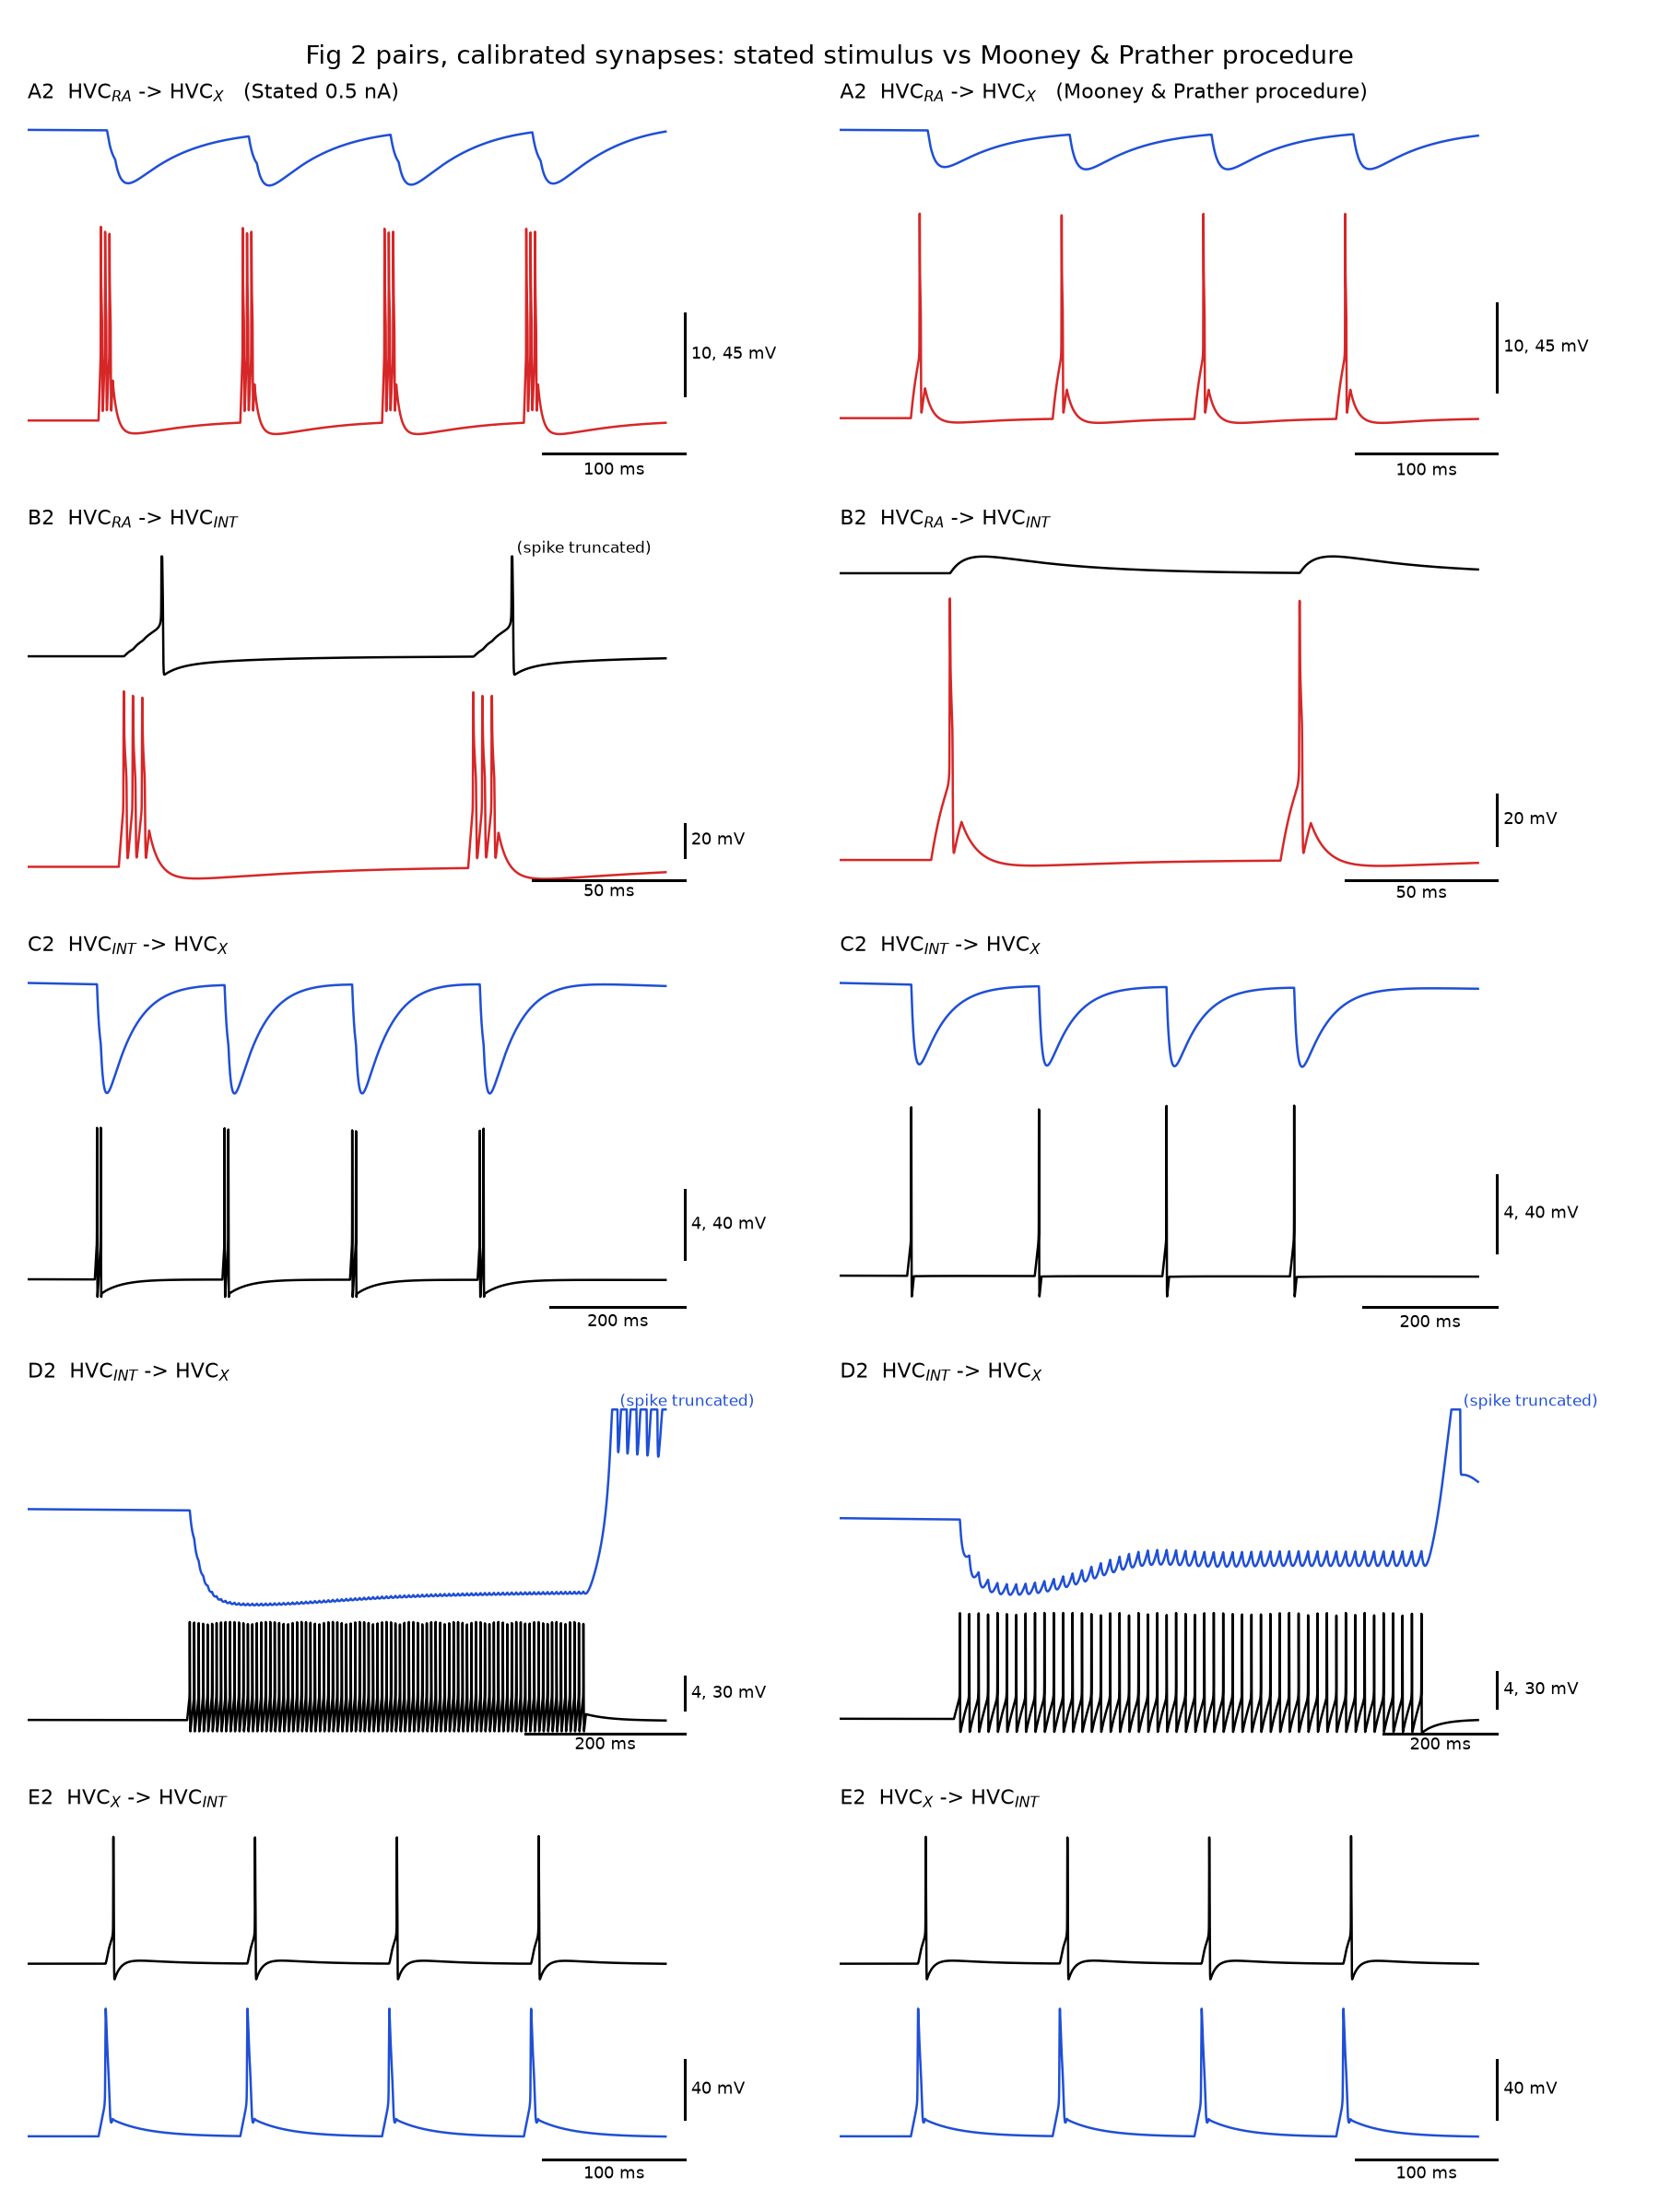
\includegraphics[width=0.9\linewidth]{figures/replication_fig2_pairs.png}
\caption{(cf.\ original Fig.~2, right column) Model pairs and the RA$\to$INT$\to$X triplet (A; the
interneuron is not drawn), with synaptic conductances fitted to the original traces. In each
panel the bottom trace is the stimulated cell. Left: the stated stimulus, 0.5\,nA (10\,ms pulses in
A, B, C, E; a 500\,ms step in D). Right: the current adjusted to give one spike per pulse, as in
Mooney \& Prather\supercite{MooneyPrather2005} (HVC\textsubscript{RA} 150\,pA, interneuron
250\,pA, HVC\textsubscript{X} 500\,pA; D: 145\,pA for 820\,ms). Pulse spacing and per-trace scale
bars as in the original panels. Postsynaptic spikes taller than three scale bars are truncated.}
\label{fig:2}\end{figure}

\begin{figure}[p]\centering
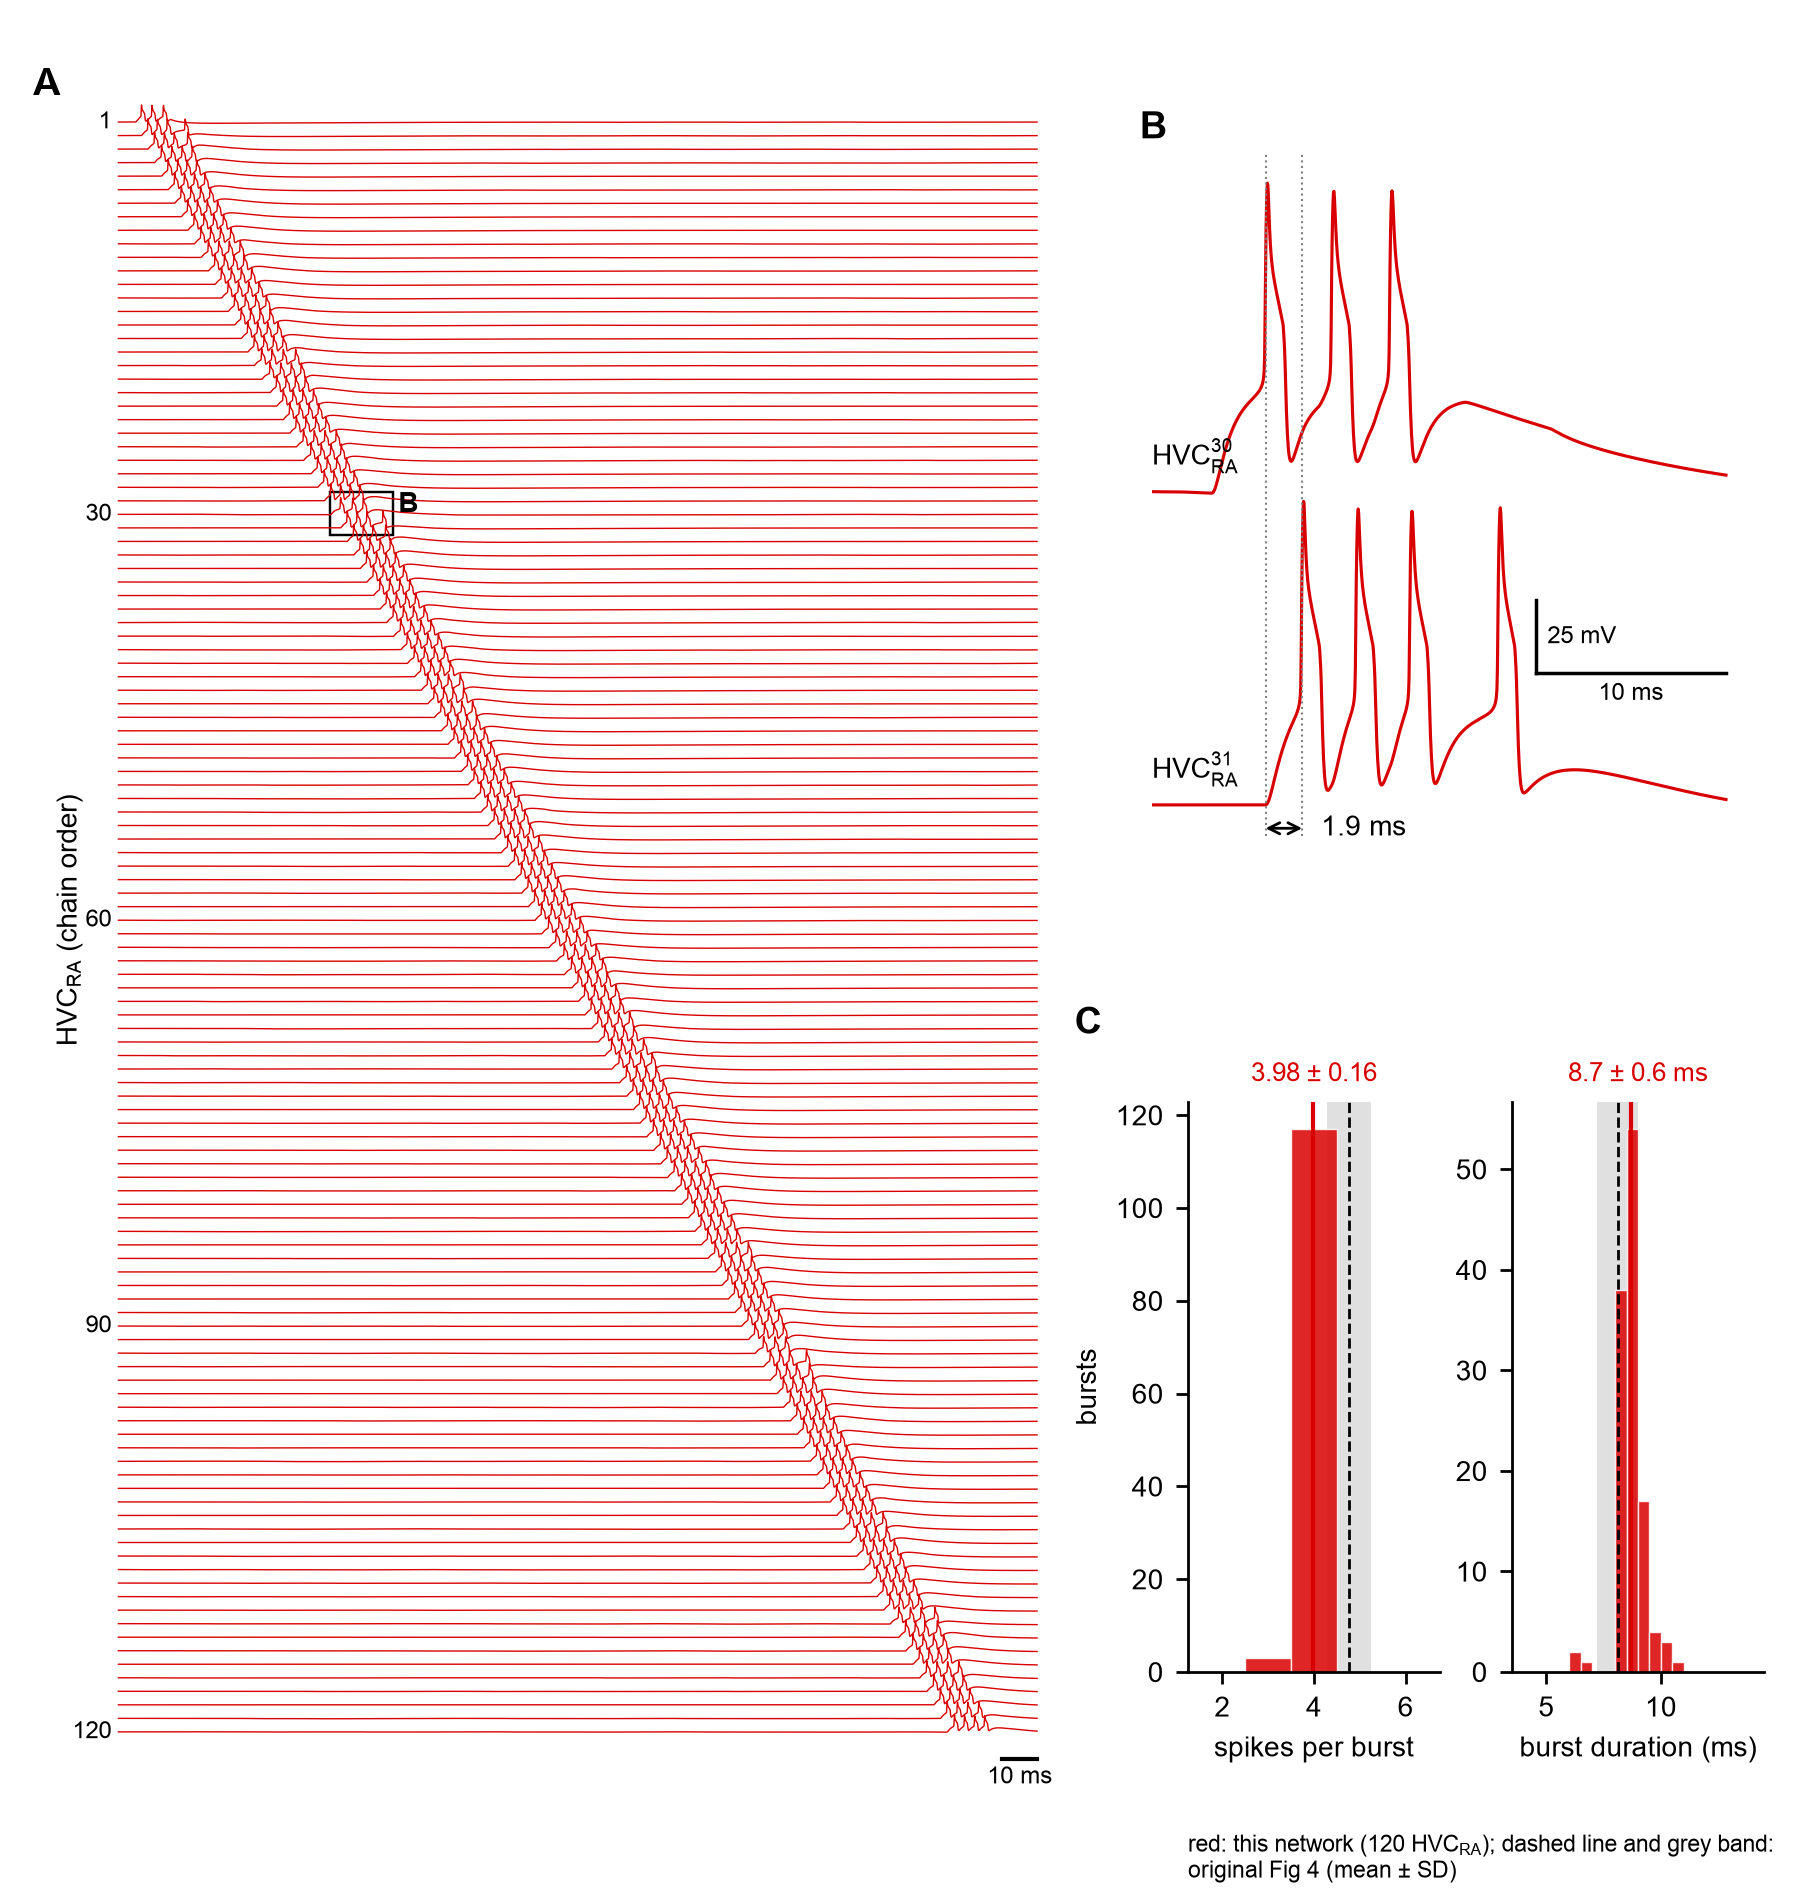
\includegraphics[width=0.85\linewidth]{figures/replication_fig4.png}
\caption{(cf.\ original Fig.~4) (A) Membrane potential of the 120 HVC\textsubscript{RA}, in chain
order, after a 500\,pA, 10\,ms pulse into the first neuron (final configuration, $C_m=20$\,pF,
network 1 of 50). (B) Enlargement of the boxed neurons 30 and 31 and the delay between their
first spikes. (C) Spikes per burst and burst duration of the 120 bursts in A (red line: mean)
against the original (dashed line: mean; grey: $\pm$1 SD).}
\label{fig:4}\end{figure}

\begin{figure}[p]\centering
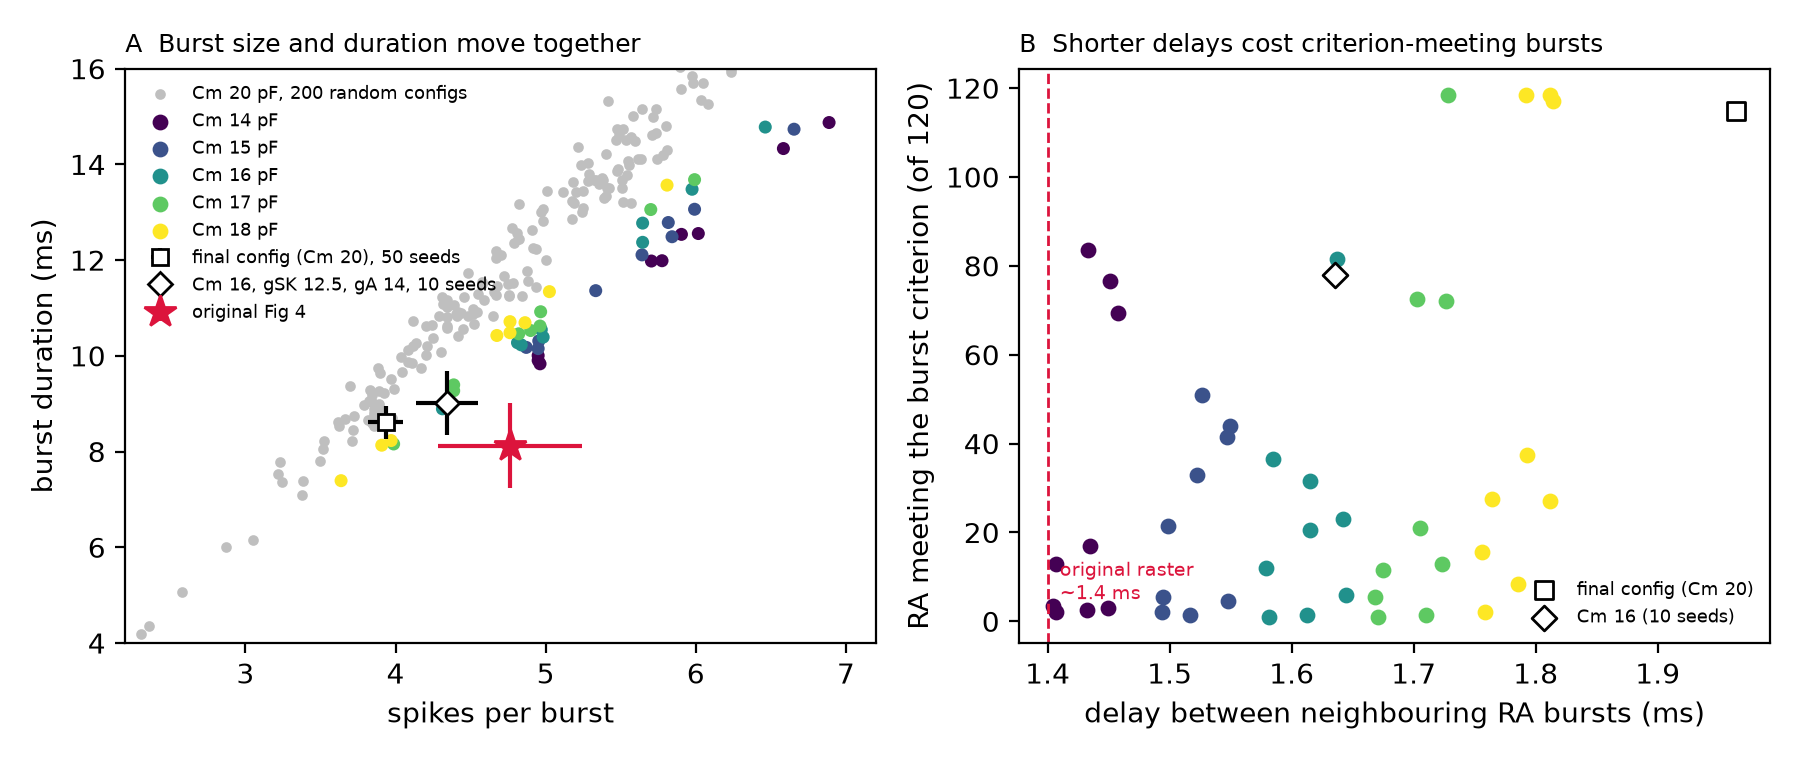
\includegraphics[width=\linewidth]{figures/article_fig4_tradeoff.png}
\caption{Fig.~4 burst statistics and the HVC\textsubscript{RA} capacitance. (A) Spikes per burst
against burst duration. Grey: 200 configurations inside the published ranges with $C_m=20$\,pF.
Coloured: full-network grid over $C_m$ 14--18\,pF, $g_{SK}$ 11--12.5\,nS and $g_A$ 5--14\,nS (2
networks each). Square: the final configuration (50 networks). Diamond: $C_m=16$\,pF,
$g_{SK}=12.5$, $g_A=14$\,nS (10 networks). Star: the original (mean $\pm$ SD). (B) Delay between
neighbouring HVC\textsubscript{RA} bursts against the number of HVC\textsubscript{RA} meeting the
burst criterion, for the same grid. Dashed line: the original raster's slope.}
\label{fig:4tradeoff}\end{figure}

\begin{figure}[p]\centering
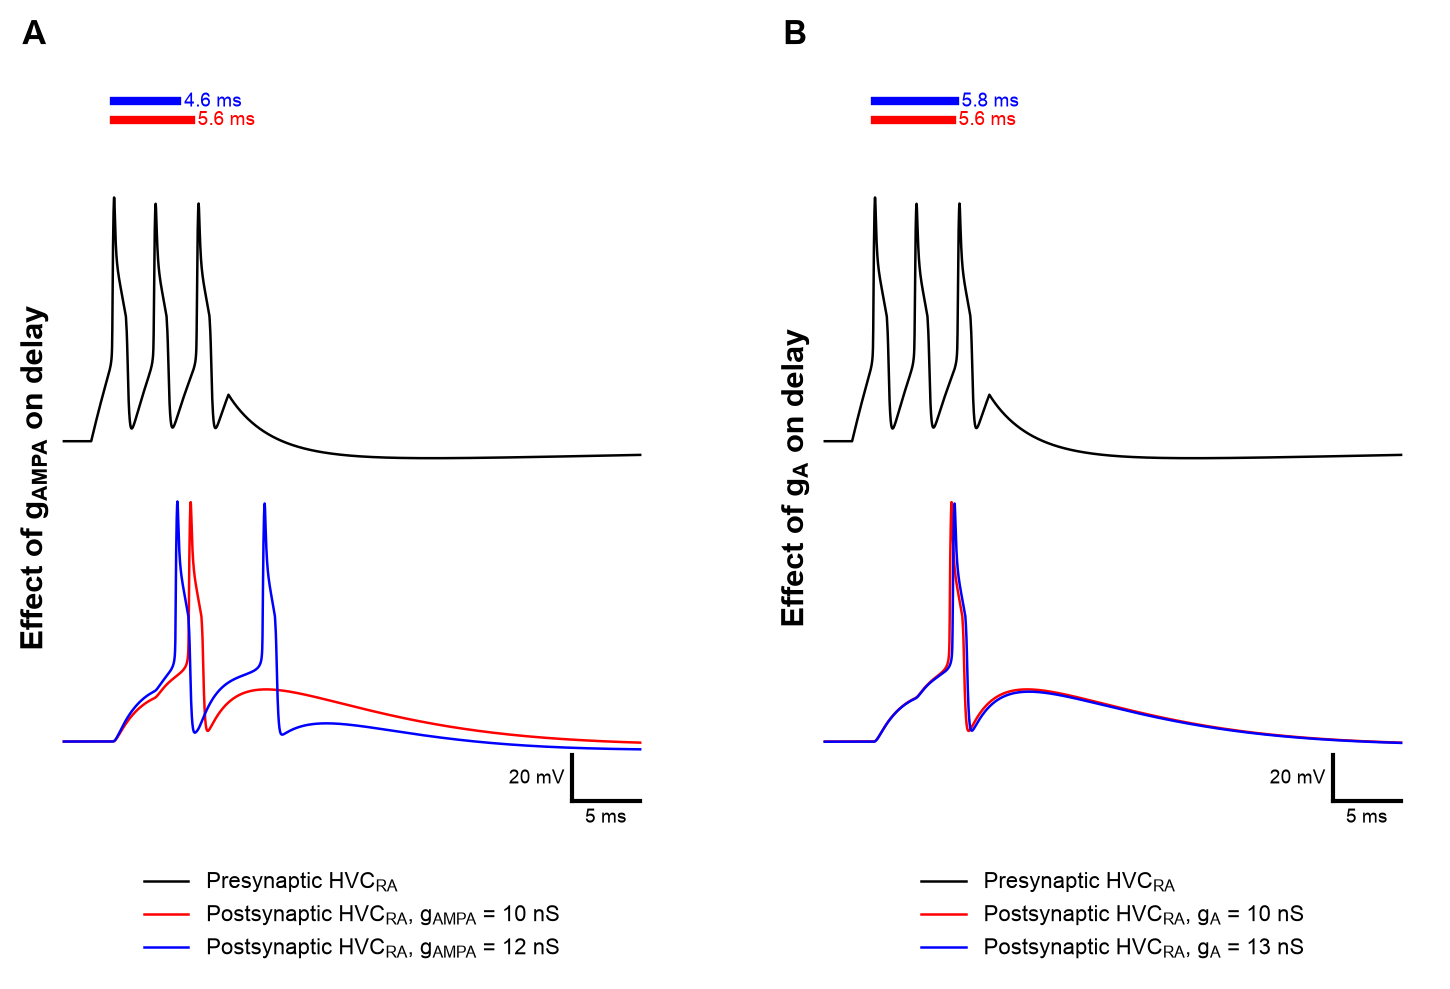
\includegraphics[width=0.95\linewidth]{figures/replication_fig5.png}
\caption{(cf.\ original Fig.~5) Effect of $g_{AMPA}$ (A) and $g_A$ (B) on the delay between
successive HVC\textsubscript{RA} bursts. Bars: first-spike-peak delay.}
\label{fig:5}\end{figure}

\begin{figure}[p]\centering
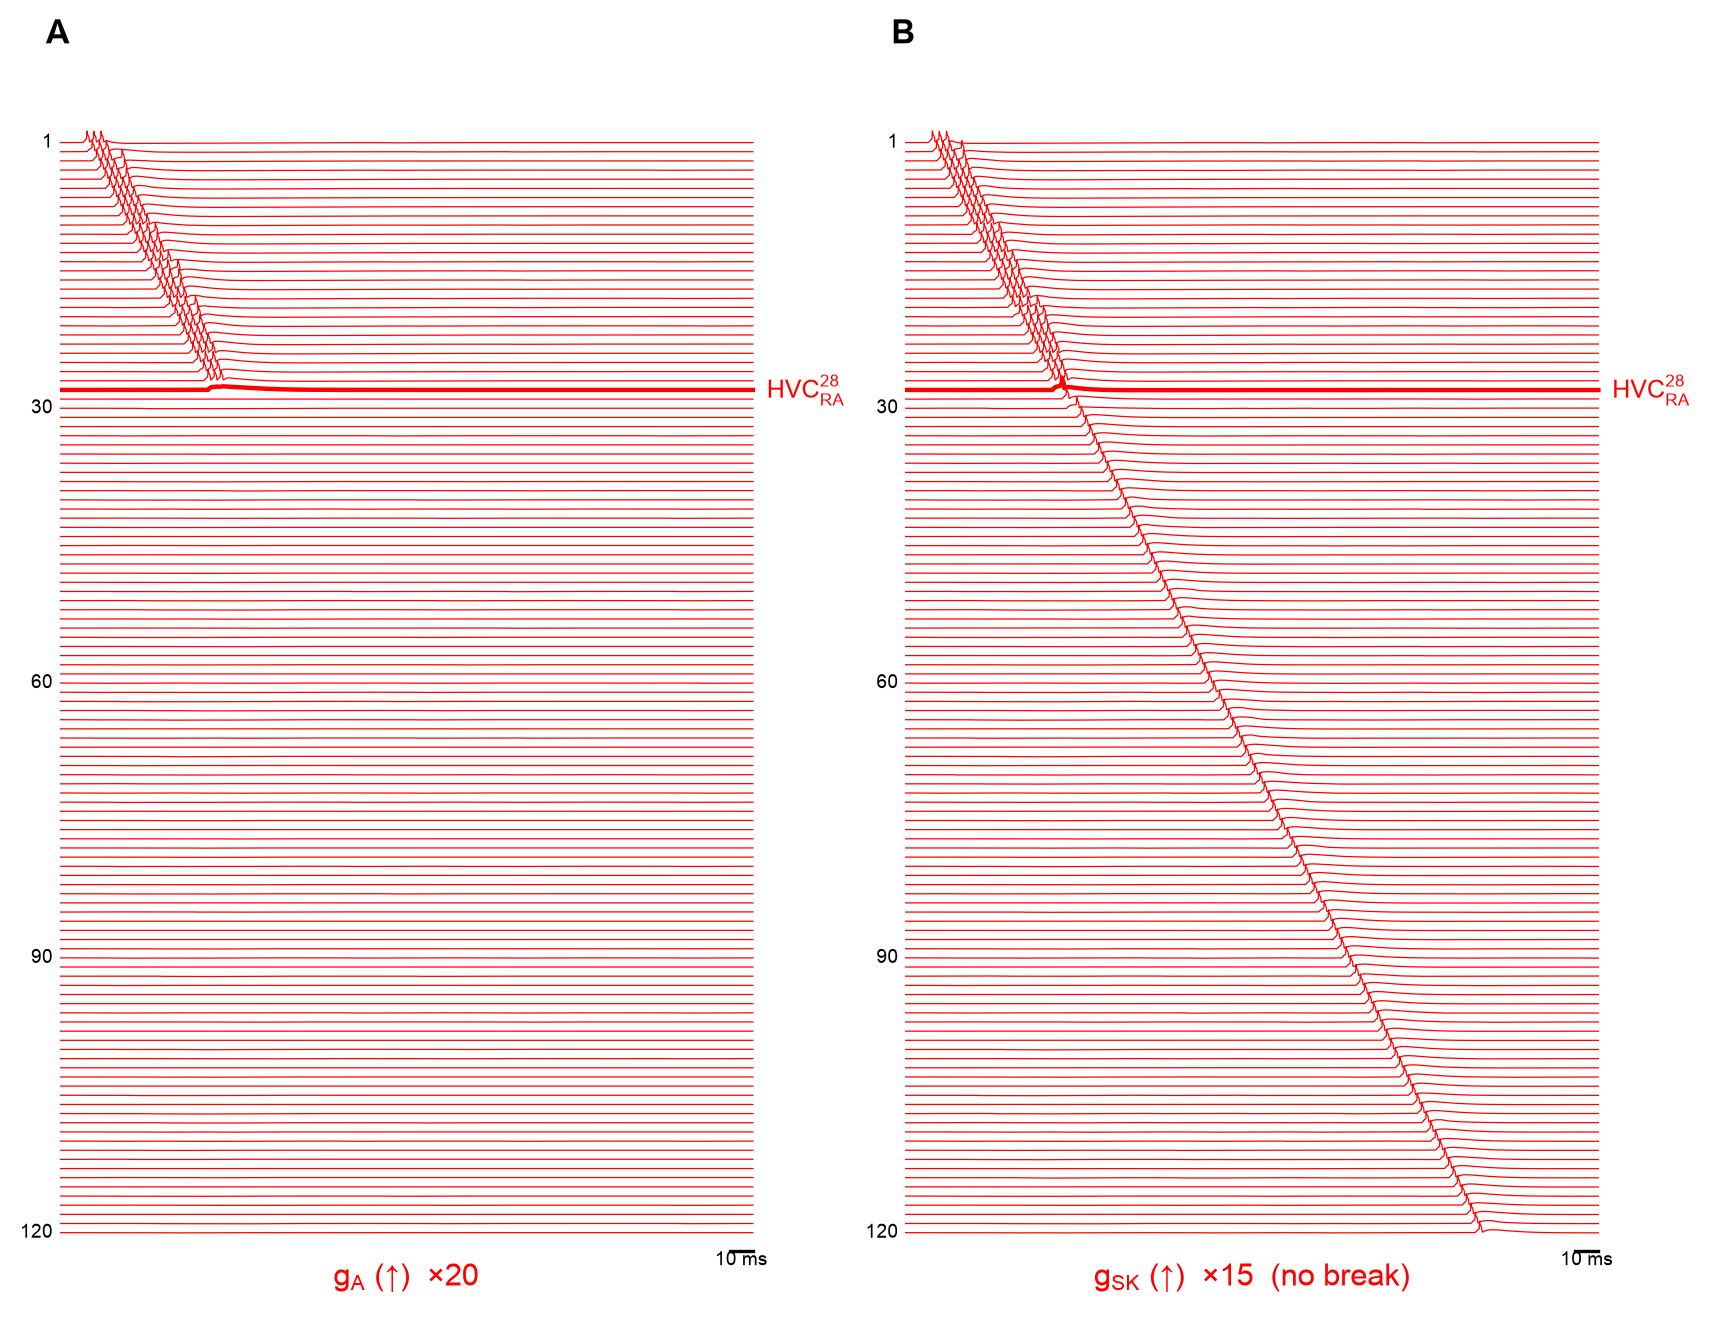
\includegraphics[width=0.95\linewidth]{figures/replication_fig6.png}
\caption{(cf.\ original Fig.~6) Up-regulating $g_A$ (A, $\times$20) or $g_{SK}$ (B, $\times$15,
the original factor) in one HVC\textsubscript{RA}, with HVC\textsubscript{INT}$\to$RA = 5\,nS.
(A) breaks the chain at the perturbed neuron. (B) reduces the perturbed neuron's burst to a
single spike, and the chain dies four neurons later; this happened in 1 of 8 trials (the one
shown).}
\label{fig:6}\end{figure}

\begin{figure}[p]\centering
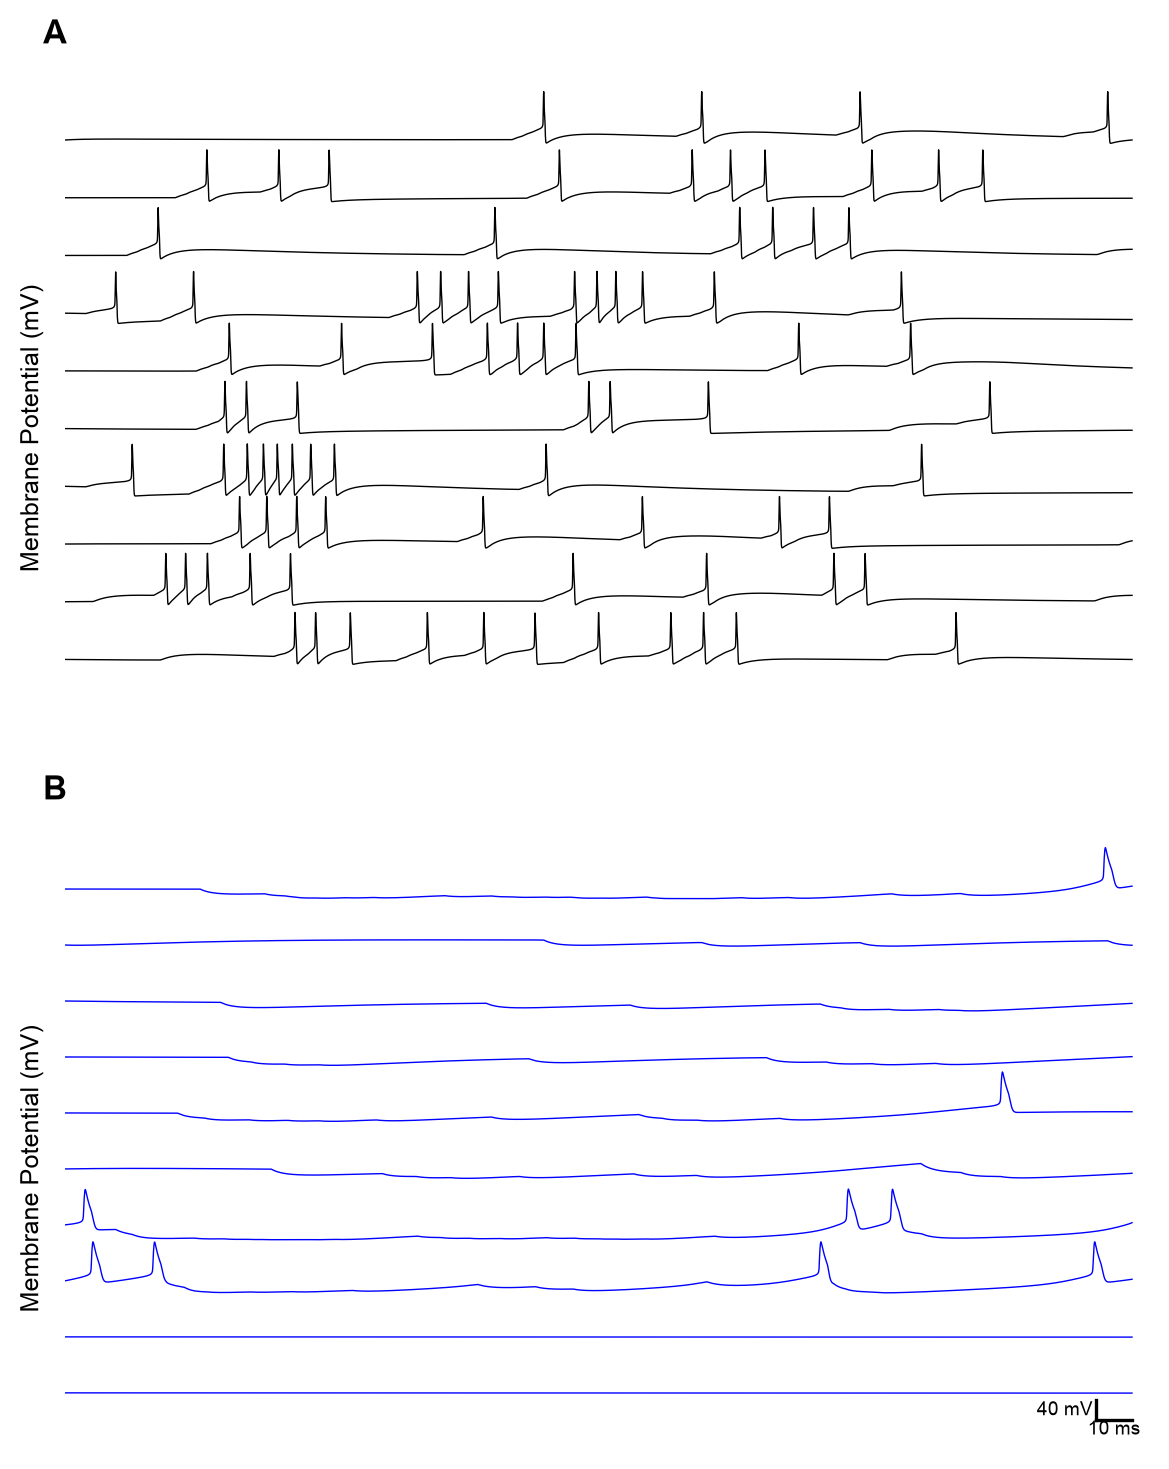
\includegraphics[width=0.7\linewidth]{figures/replication_fig7.png}
\caption{(cf.\ original Fig.~7) Activity of 10 HVC\textsubscript{INT} (A) and 10
HVC\textsubscript{X} (B). Interneurons fire sparsely, and HVC\textsubscript{X} fire isolated
rebound spikes rather than 2--4 rebound bursts.}
\label{fig:7}\end{figure}

\begin{figure}[p]\centering
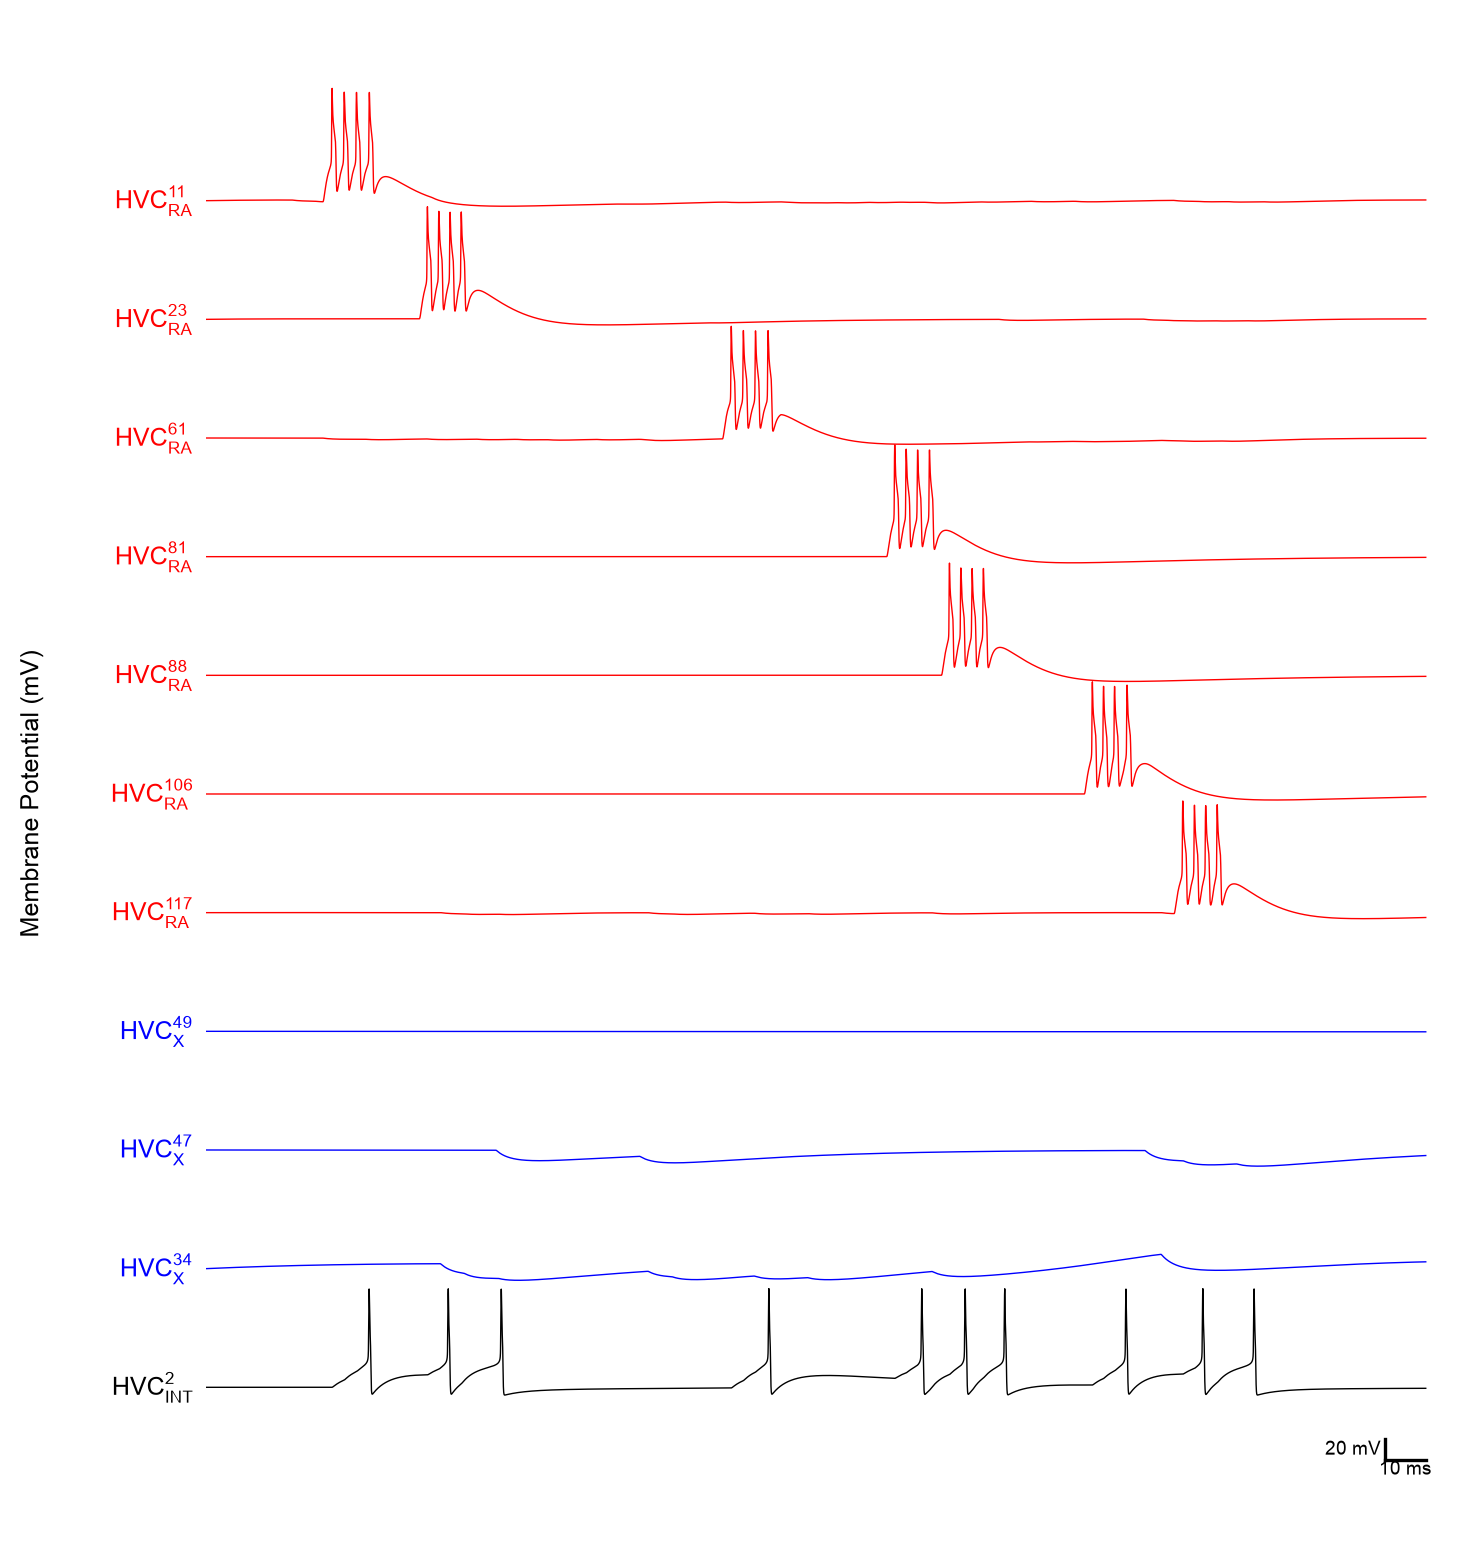
\includegraphics[width=0.8\linewidth]{figures/replication_fig8.png}
\caption{(cf.\ original Fig.~8) One interneuron with its presynaptic HVC\textsubscript{RA}
(red) and HVC\textsubscript{X} (blue). Its spikes align with its HVC\textsubscript{RA} inputs,
but it doesn't burst densely.}
\label{fig:8}\end{figure}

\begin{figure}[p]\centering
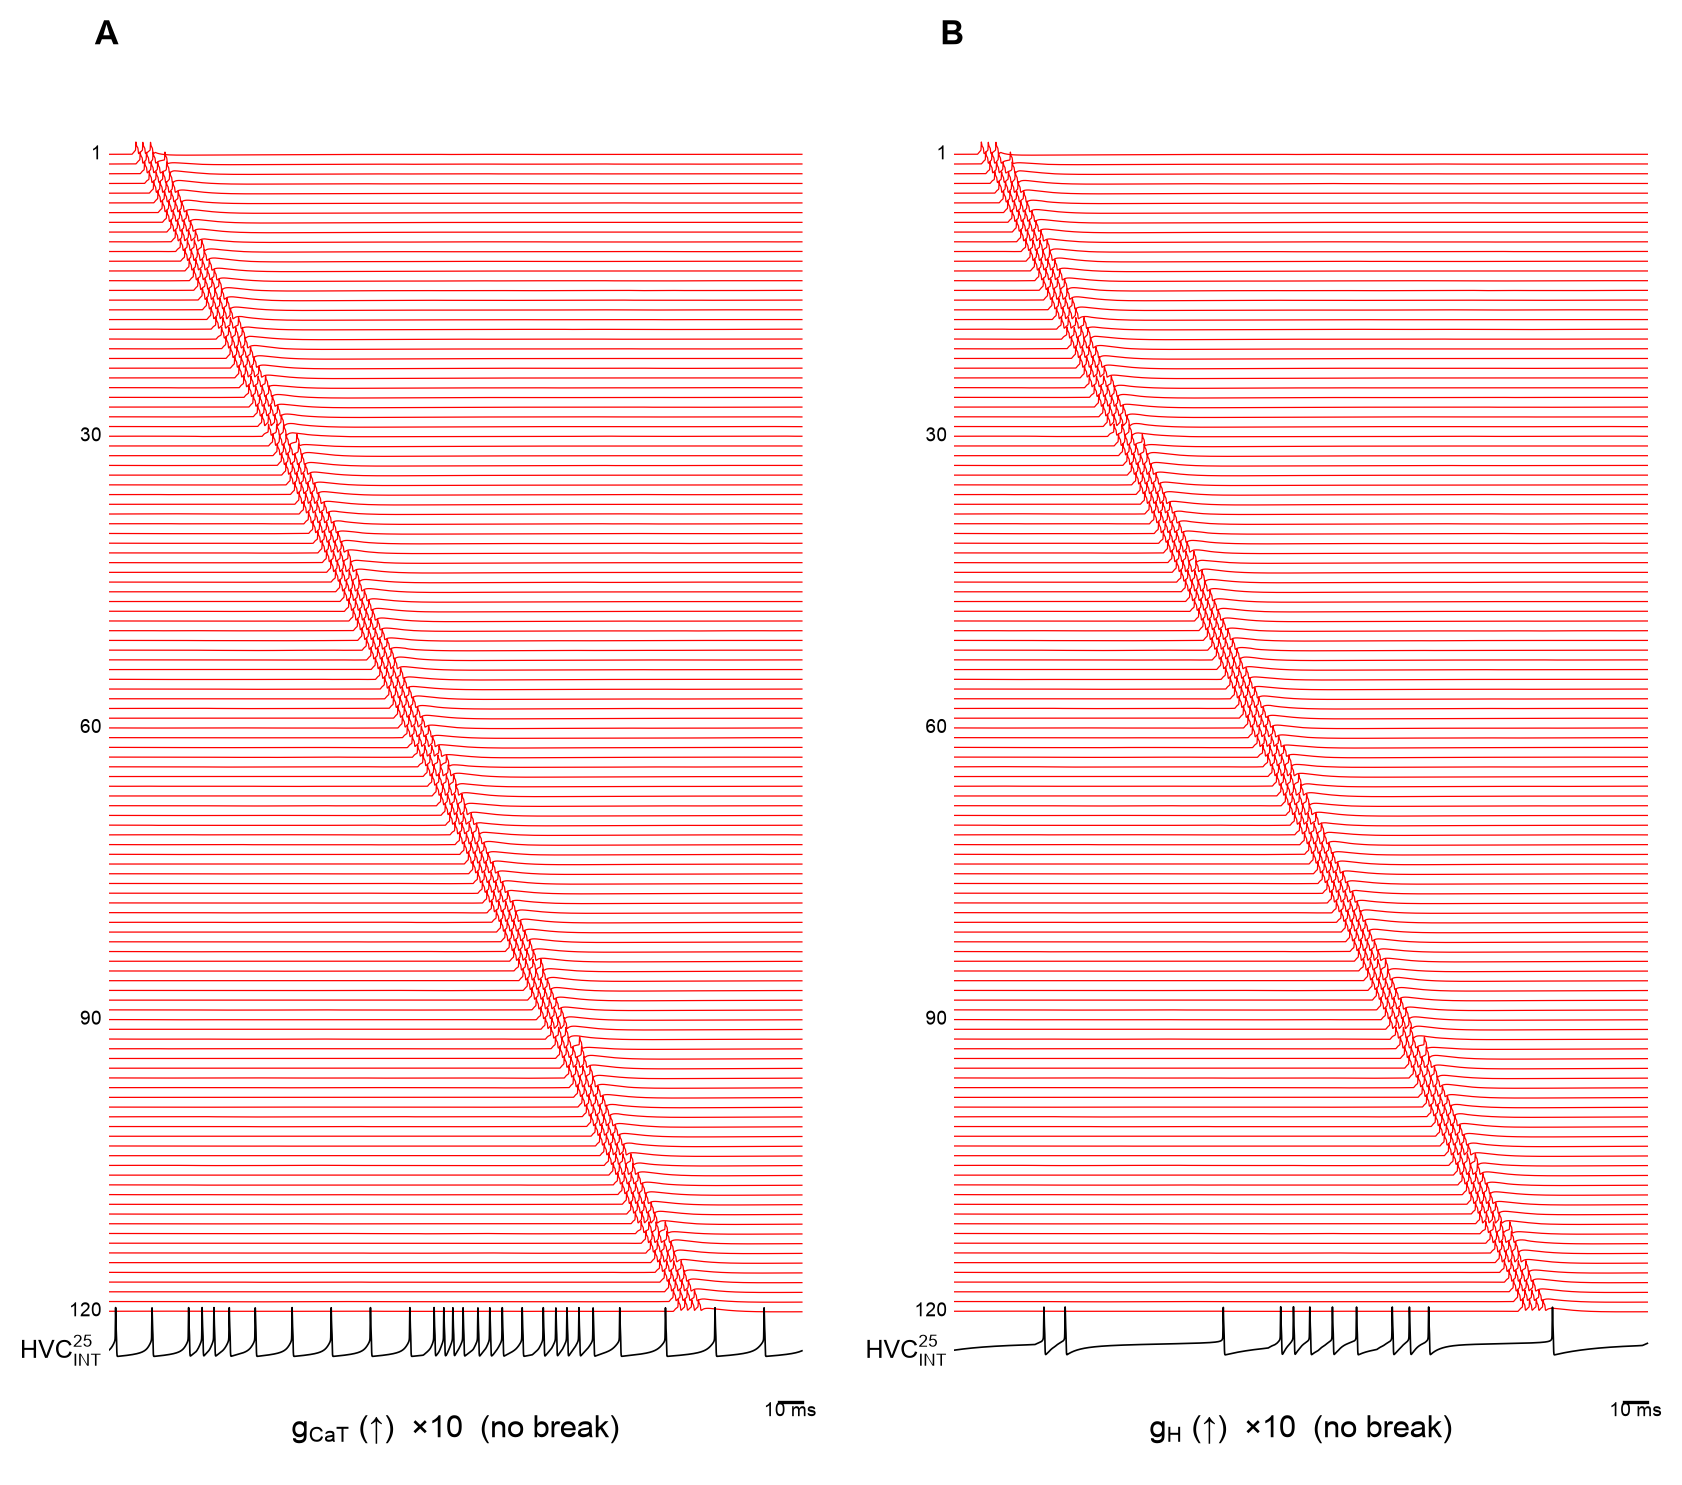
\includegraphics[width=0.95\linewidth]{figures/replication_fig9.png}
\caption{(cf.\ original Fig.~9) Up-regulating $g_{CaT}$ (A) or $g_H$ (B) 10$\times$ in one
interneuron (bottom trace). The interneuron fires more, but the chain does not break.}
\label{fig:9}\end{figure}

\begin{figure}[p]\centering
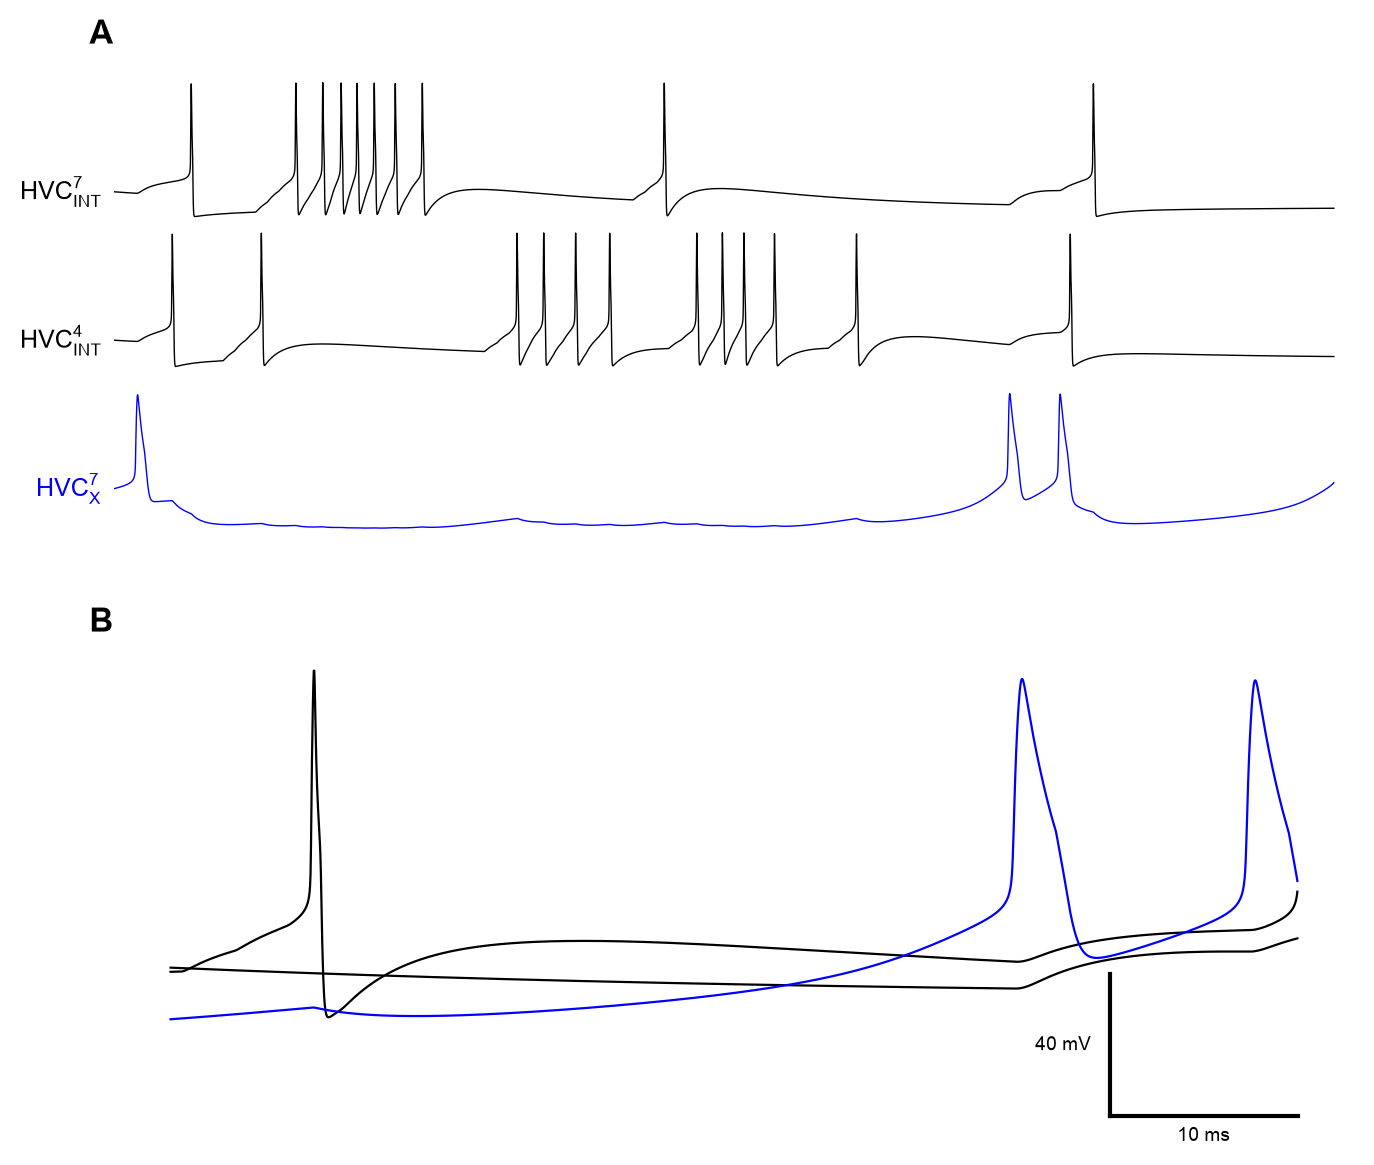
\includegraphics[width=0.8\linewidth]{figures/replication_fig10.png}
\caption{(cf.\ original Fig.~10) An HVC\textsubscript{X} and its presynaptic interneurons (A),
with a 60\,ms zoom (B). HVC\textsubscript{X} escape inhibition with single spikes.}
\label{fig:10}\end{figure}

\begin{figure}[p]\centering
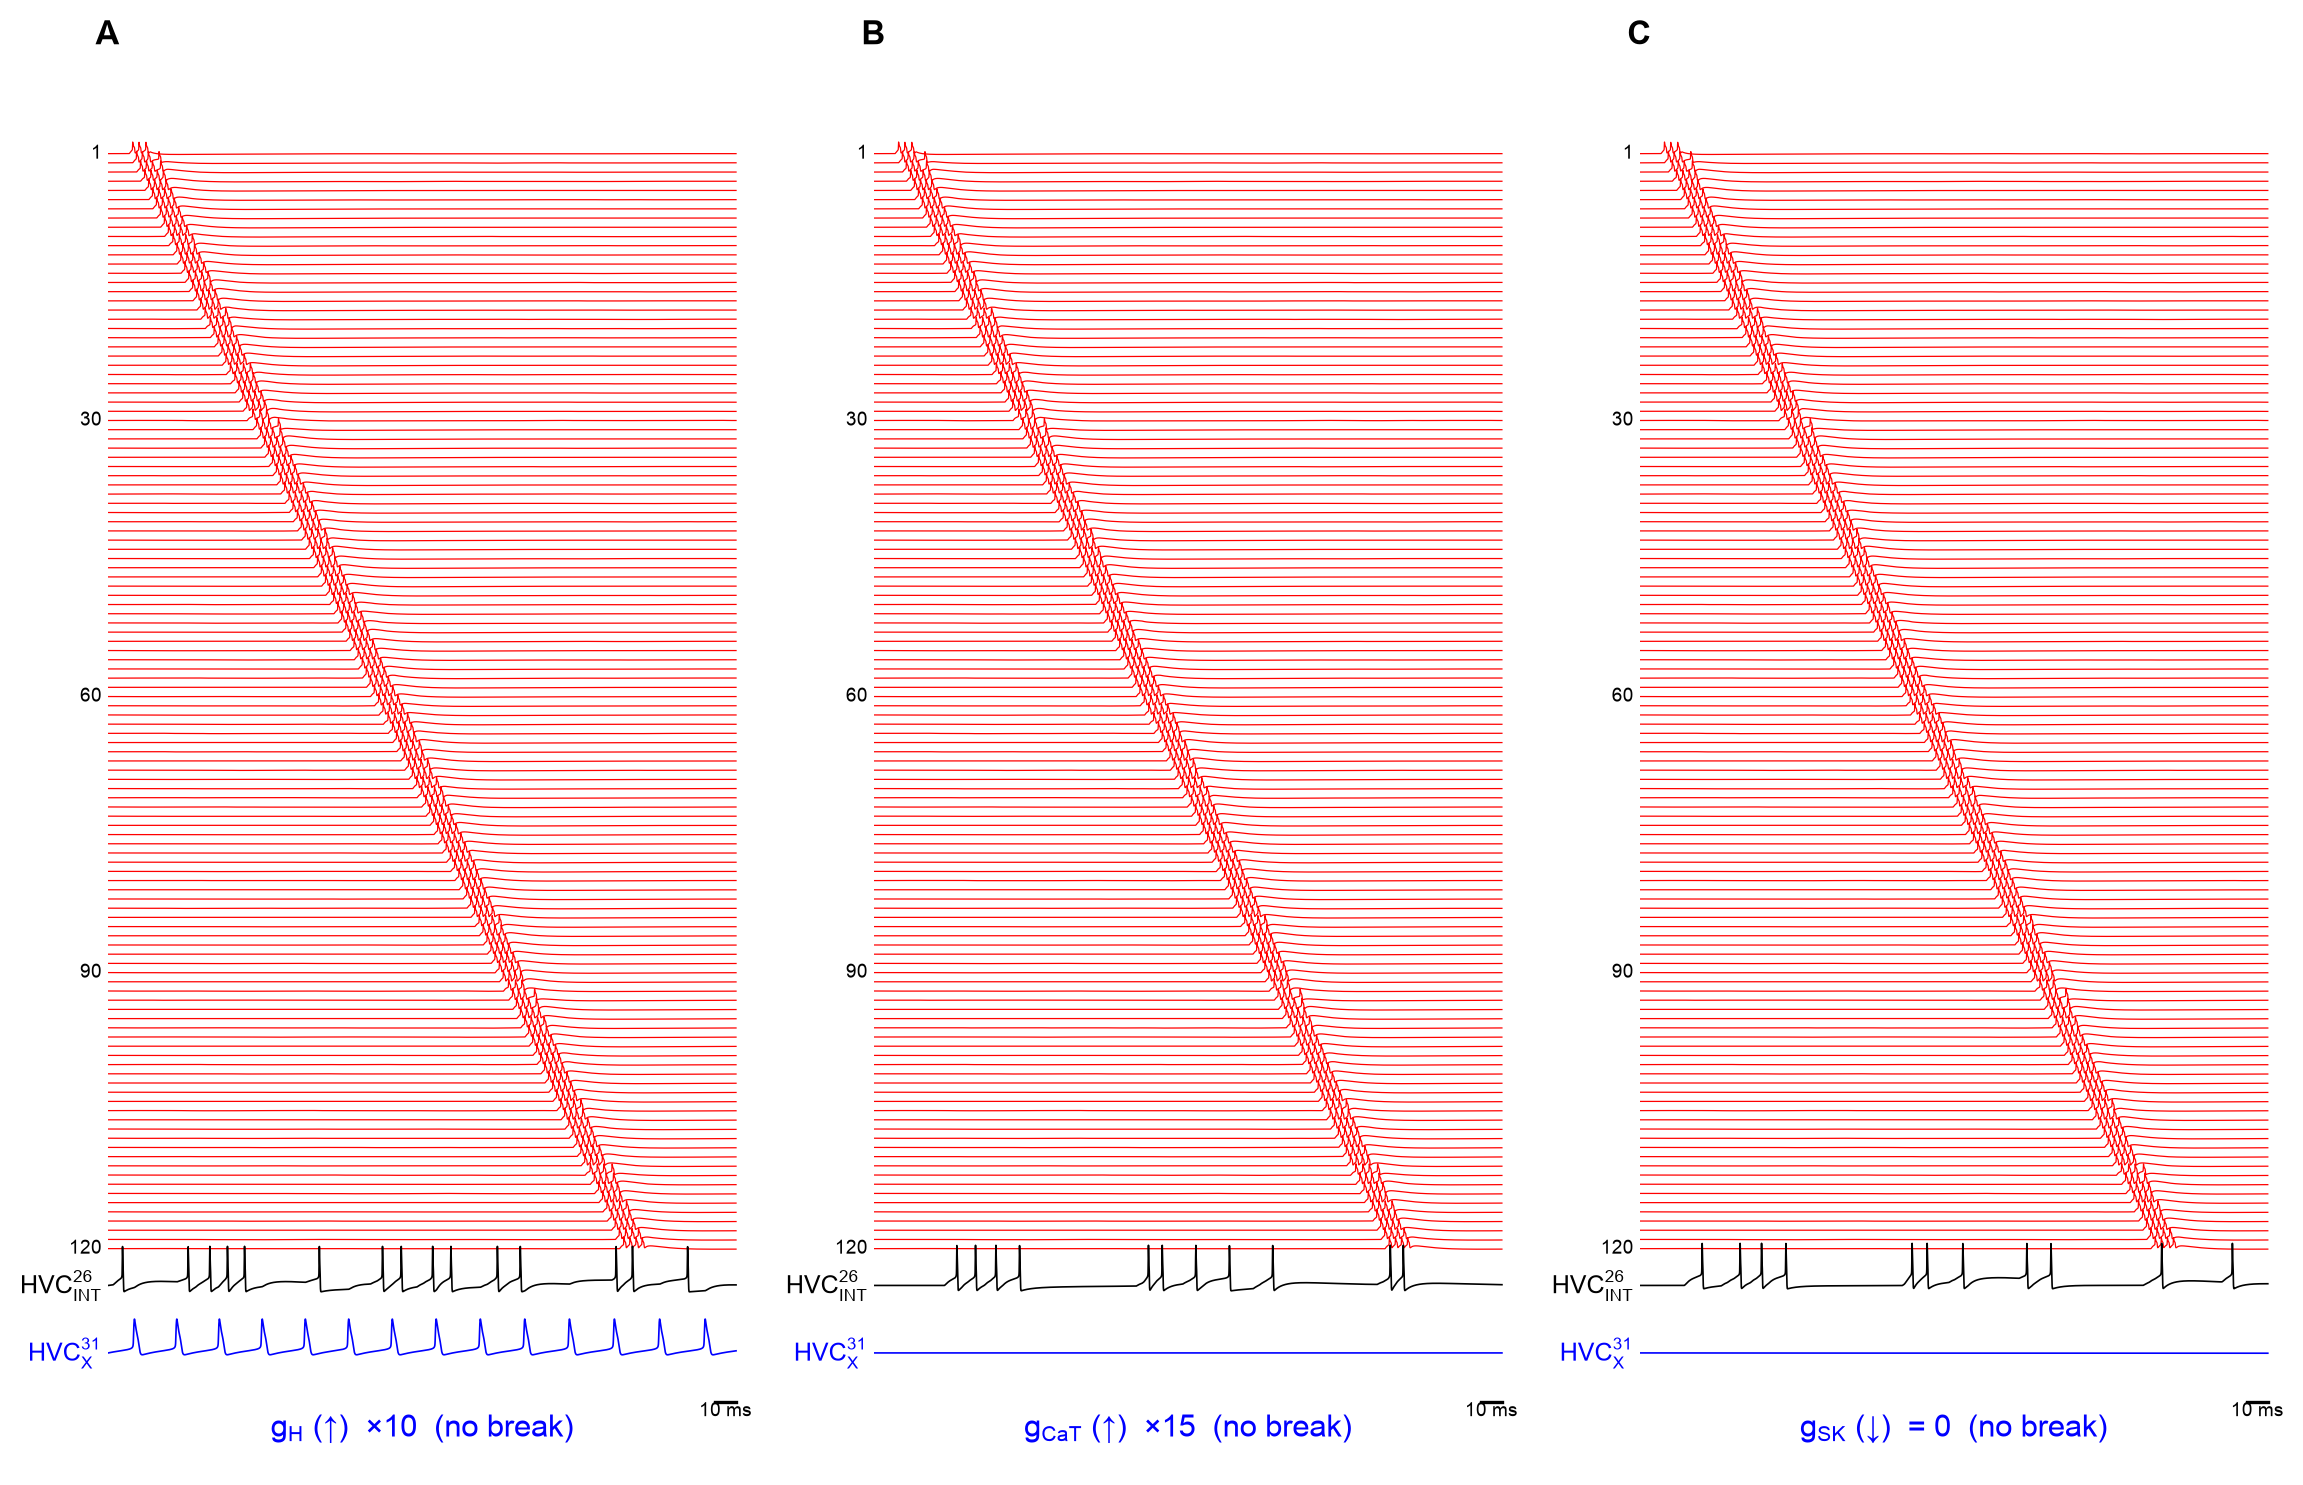
\includegraphics[width=\linewidth]{figures/replication_fig11.png}
\caption{(cf.\ original Fig.~11) HVC\textsubscript{X} perturbations: $g_H$ $\times$10 (A),
$g_{CaT}$ $\times$15 (B), $g_{SK}=0$ (C). The bottom traces show the perturbed
HVC\textsubscript{X} and an interneuron it excites. The chain does not break.}
\label{fig:11}\end{figure}

\begin{figure}[p]\centering
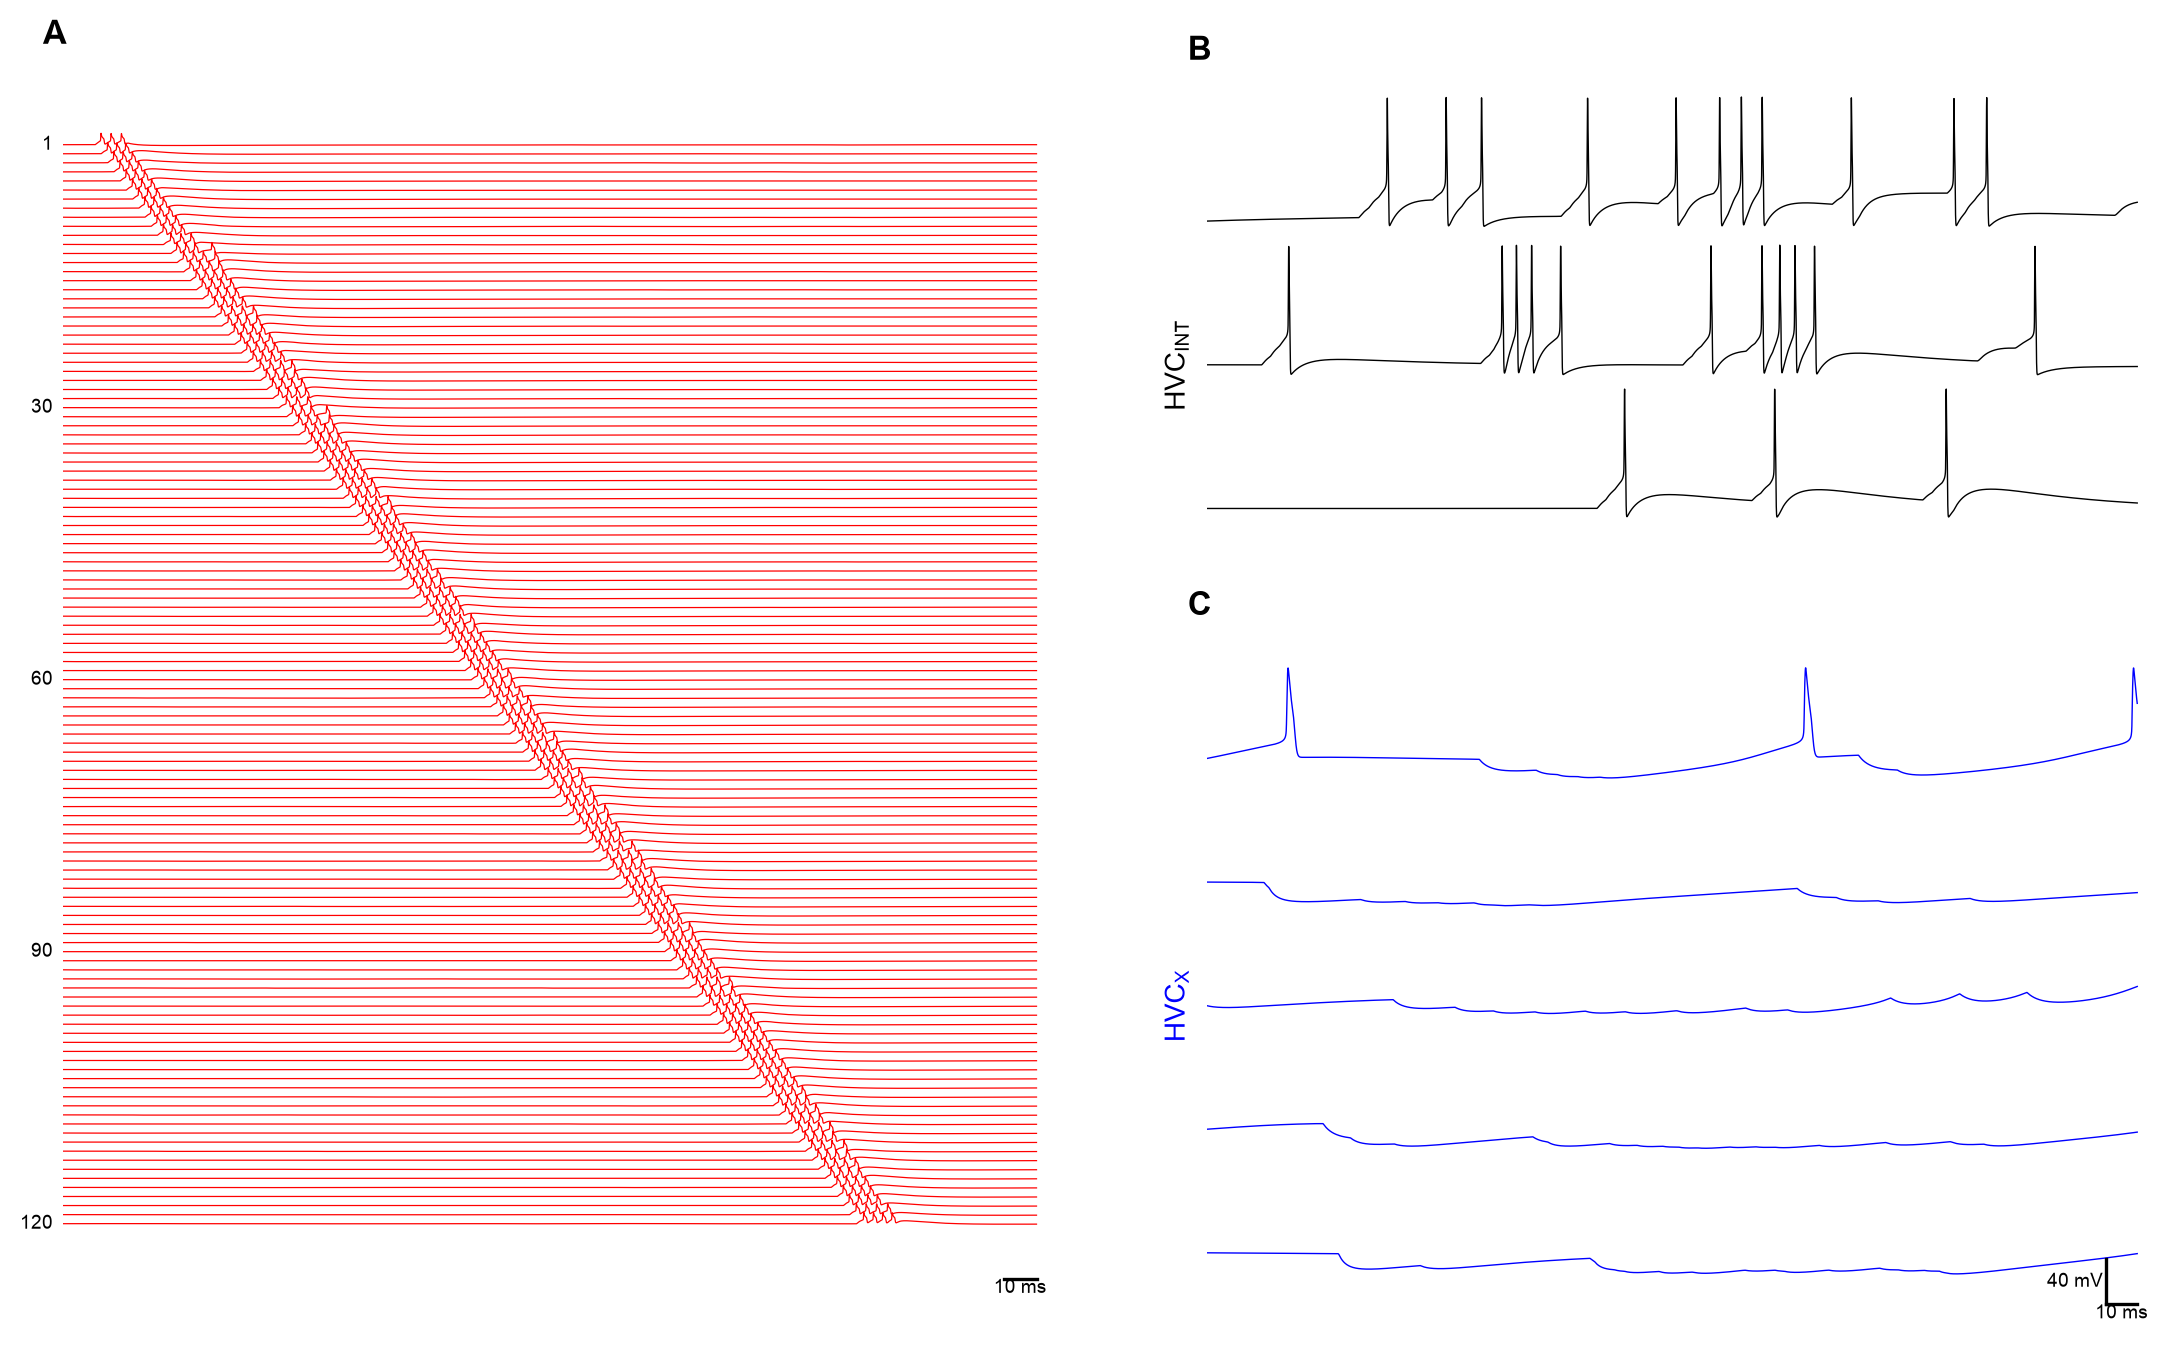
\includegraphics[width=\linewidth]{figures/replication_fig12.png}
\caption{(cf.\ original Fig.~12) Example with HVC\textsubscript{X} conductances drawn per neuron
within the published ranges. (A) HVC\textsubscript{RA}, (B) interneurons, (C)
HVC\textsubscript{X}. None of 100 such runs broke the chain.}
\label{fig:12}\end{figure}

\begin{figure}[p]\centering
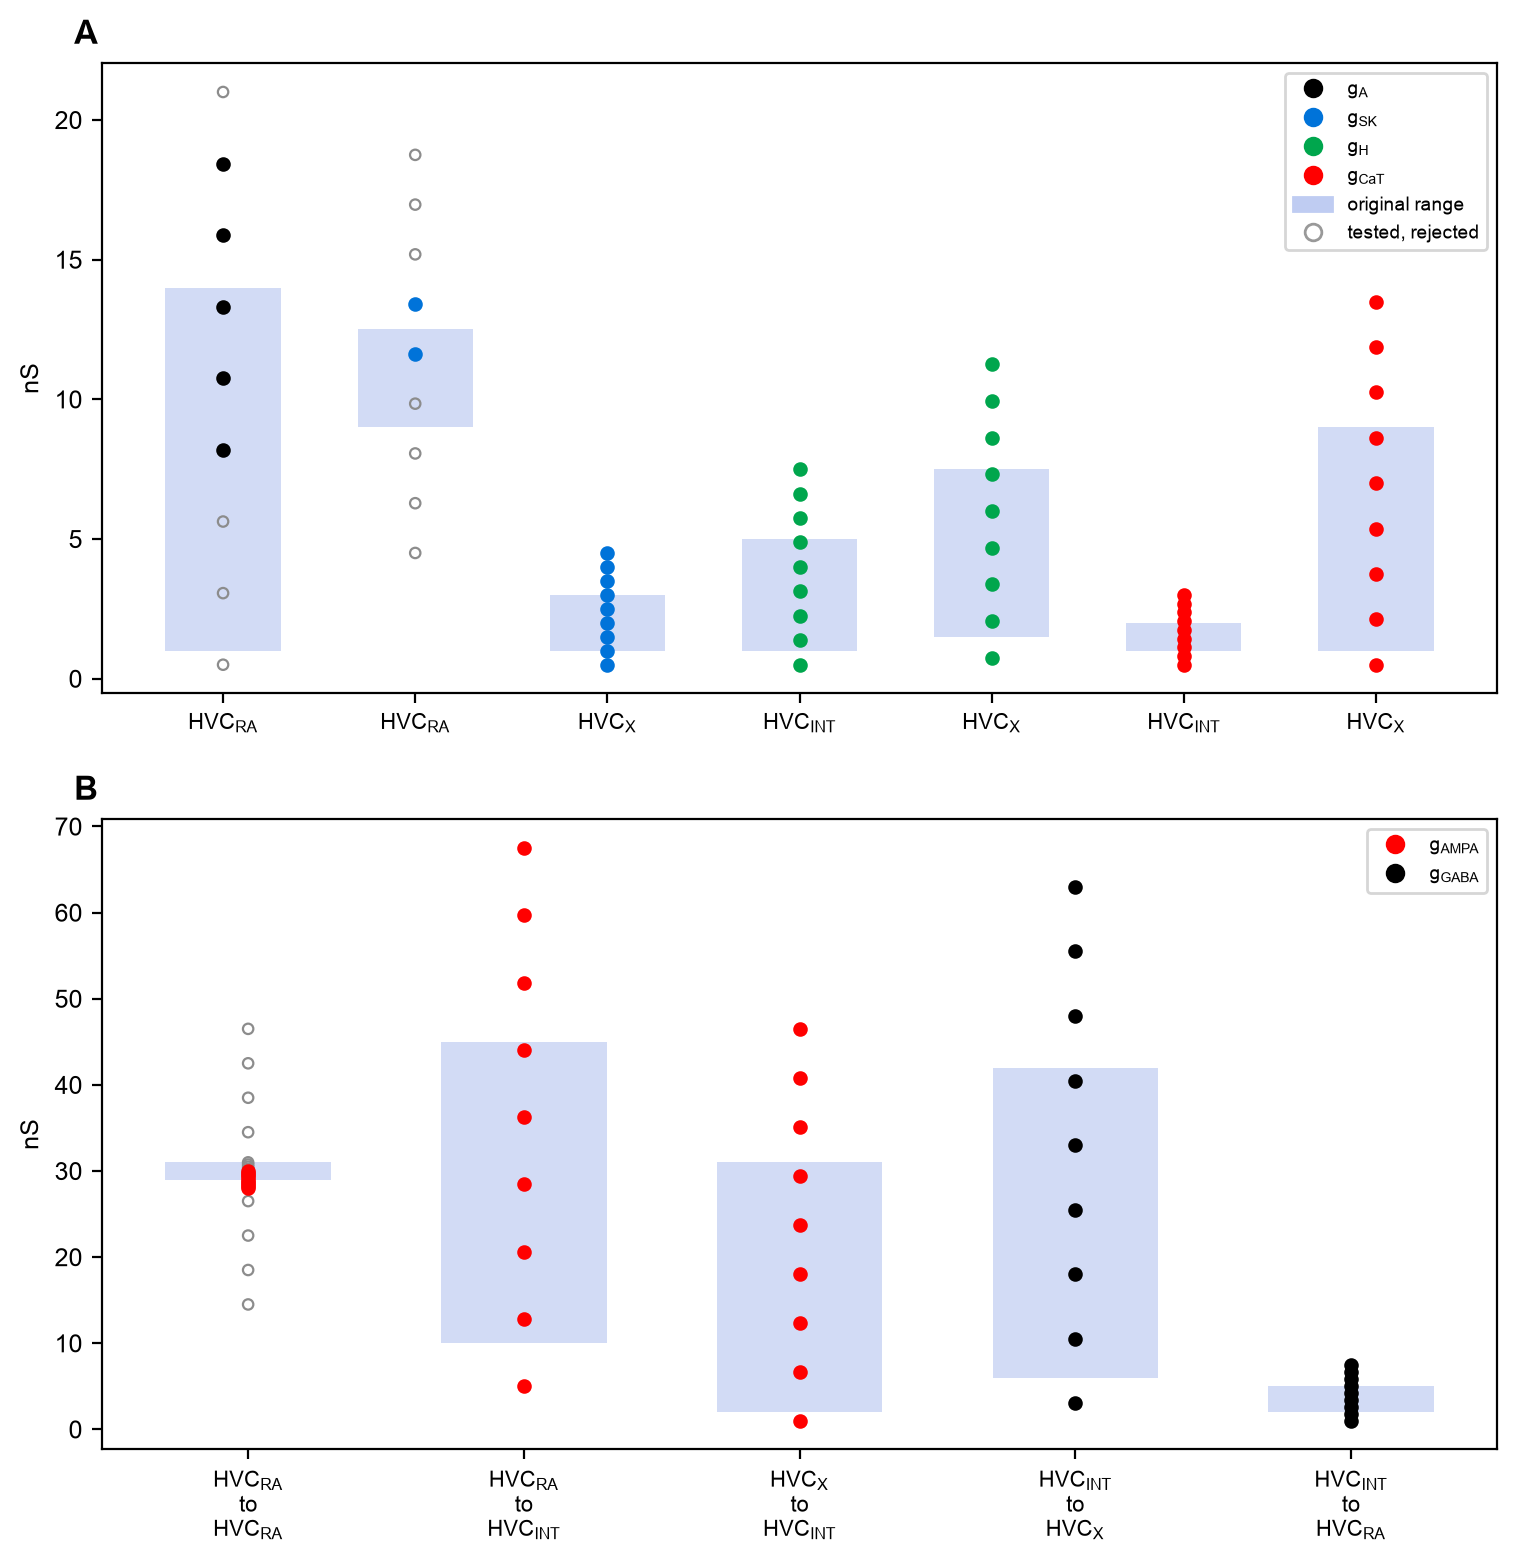
\includegraphics[width=0.8\linewidth]{figures/replication_fig13.png}
\caption{(cf.\ original Fig.~13) Ionic (A) and synaptic (B) conductances varied one at a time
around the final configuration (2 seeds). Shaded: the original allowed range. Filled: values
for which the chain completes and $\geq$90/120 HVC\textsubscript{RA} meet the burst criterion in
both seeds. Open: rejected values.}
\label{fig:13}\end{figure}

\begin{figure}[p]\centering
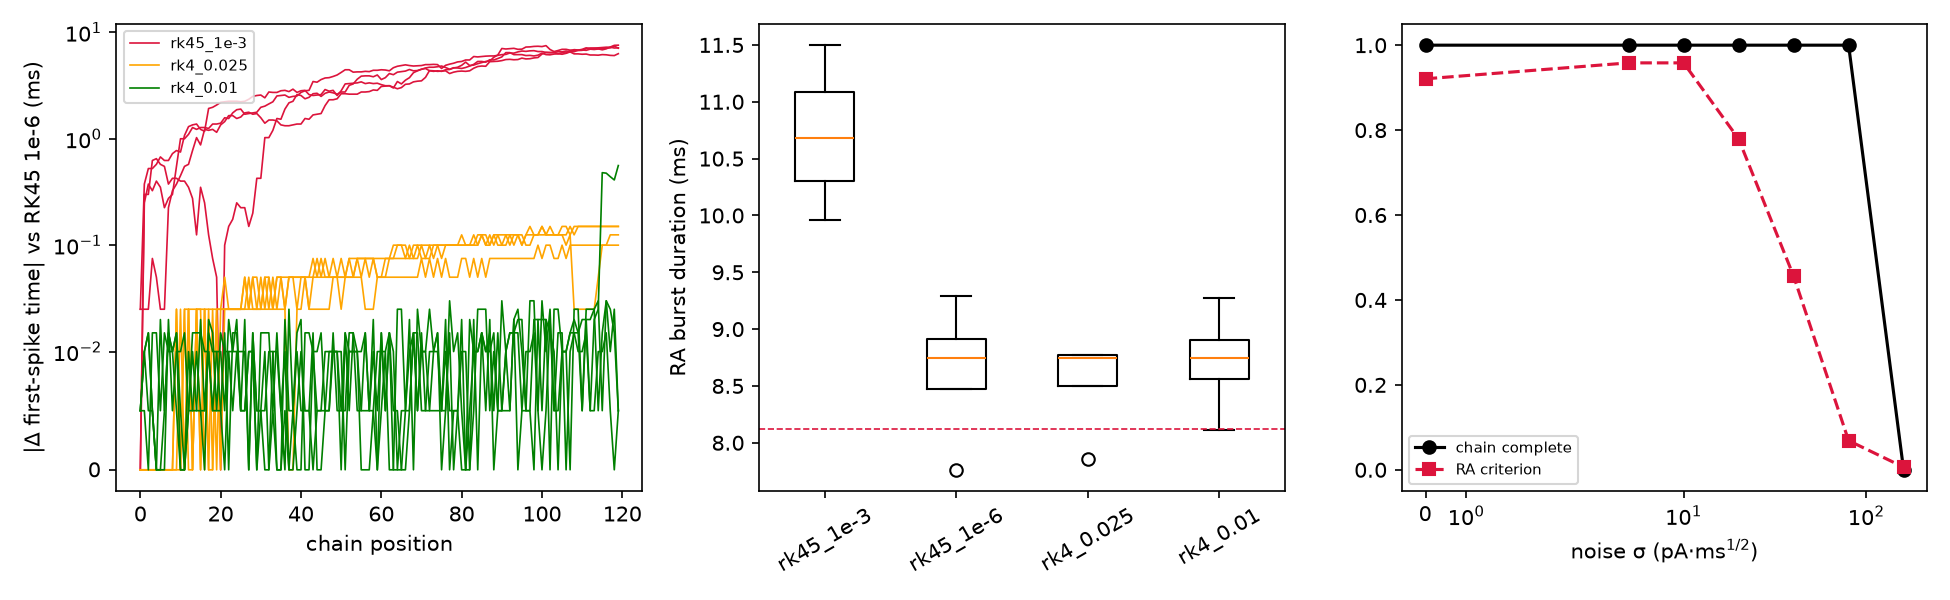
\includegraphics[width=\linewidth]{figures/article_numerics_noise.png}
\caption{Numerics and noise (not in the original). Left: first-spike-time deviation from RK45
($10^{-6}$) along the chain for RK45 at MATLAB-default tolerance and RK4 at 0.025/0.01\,ms.
Middle: burst duration by solver (dashed: original mean). Right: chain completion and burst
criterion against noise amplitude.}
\label{fig:num}\end{figure}

\section*{Reproducibility notes}
\begin{table}[h]\small
\caption{Main corrections and open choices. The full log of $\sim$45 items is in the repository
(\texttt{notes/issues-log.md}).}
\label{tab:issues}
\begin{tabular}{p{0.32\linewidth}p{0.6\linewidth}}
\hline
Item (Appendix~1) & Used here \\ \hline
Eq.~9: $(x_\infty - V)/\tau_x$ & $(x_\infty - x)/\tau_x$ (Daou 2013) \\
$\tau_n$ constant 10\,ms & $\bar\tau_n/\cosh((V-\theta_n)/2\sigma_n)$ (Daou 2013); the constant gives 10\,ms spikes \\
Eq.~17: $r_{T\infty}$ uses $\theta_{aT},\sigma_{aT}$ & $\theta_{rT}=-67$, $\sigma_{rT}=2$ (Daou 2013) \\
Eq.~21: $+k_{Ca}([Ca]-b_{Ca})$ & $-f[\varepsilon(I_{CaL}+I_{CaT})+k_{Ca}([Ca]-b_{Ca})]$ (Daou 2013) \\
GHK currents without a $V$ factor & $g\,x\,V\,Ca_{ex}/(1-e^{2V/RTF})$ (Daou 2013) \\
$r_{s\infty}$ sign (activates on depolarisation) & sign as in Daou 2013 code \\
$\sigma_{aT}=+7.8$ & $-7.8$ (Daou 2013) \\
Transmitter release sign & $T_{max}/(1+e^{-(V_{pre}-V_T)/K_p})$ (Destexhe 1994) \\
$C_m$, $Ca_{ex}$, $k_r$, $T$ not given & Daou 2013: $C_m$ 20/100/75\,pF, 2.5\,mM, $k_r$ 0.3/0.01, $RT/F$ 25.7\,mV \\
$V_{AMPA}$, $V_{GABA}$ not given & 0, $-80$\,mV (Destexhe 1994) \\
Default $\bar g$ values not given & calibrated within the Fig.~13 ranges (Methods) \\
Solver tolerances, seeds, start pulse & rtol $10^{-6}$, including the 500\,ms settling; seeds in repository; 500\,pA, 10\,ms into HVC\textsubscript{RA}1 only \\
Noise ``1--5\% of the mean synaptic conductance'' (units unclear; on or off in main figures unclear) & off in main runs; amplitude swept in Robustness \\
ODE counts 6/8/7 vs Eqs.~1--3 (5/7/7) & currents as in Eqs.~1--3 \\
Supplementary code & network files are a template (no HVC\textsubscript{X}, no RA$\leftrightarrow$INT synapses); ODE file identical to Daou 2013 \\ \hline
\end{tabular}
\end{table}

\section*{Acknowledgements}
We thank the authors of the original article for publishing it with open review, and Daou et
al.\ for making their 2013 single-cell code available. This work received no funding. Code was
written and analyses were run with the assistance of an AI coding assistant (Claude, Anthropic).
The author checked and takes responsibility for all code, results and text.
